%
% File emnlp2018.tex
%
%% Based on the style files for EMNLP 2018, which were
%% Based on the style files for ACL 2018, which were
%% Based on the style files for ACL-2015, with some improvements
%%  taken from the NAACL-2016 style
%% Based on the style files for ACL-2014, which were, in turn,
%% based on ACL-2013, ACL-2012, ACL-2011, ACL-2010, ACL-IJCNLP-2009,
%% EACL-2009, IJCNLP-2008...
%% Based on the style files for EACL 2006 by 
%%e.agirre@ehu.es or Sergi.Balari@uab.es
%% and that of ACL 08 by Joakim Nivre and Noah Smith

\documentclass[11pt,a4paper]{article}
\usepackage[hyperref]{emnlp2018}
% \hypersetup{draft}
\usepackage{times}
\usepackage{latexsym}
\usepackage{amsmath}
\usepackage{amssymb}
\usepackage{graphicx}
\usepackage{url}
\usepackage{enumitem}
\usepackage{comment}
\usepackage{tabularx}
\usepackage{xcolor}
\usepackage{subcaption}

\aclfinalcopy % Uncomment this line for the final submission
%\def\aclpaperid{***} %  Enter the acl Paper ID here

%\setlength\titlebox{5cm}
% You can expand the titlebox if you need extra space
% to show all the authors. Please do not make the titlebox
% smaller than 5cm (the original size); we will check this
% in the camera-ready version and ask you to change it back.

\newcommand\BibTeX{B{\sc ib}\TeX}
\newcommand\confname{EMNLP 2018}
\newcommand\conforg{SIGDAT}
\renewcommand{\quote}{\list{}{\rightmargin=0pt\leftmargin=0pt\topsep=3pt}\item\relax}

% bcw: or something
% It actually sound really nice
\title{Learning Disentangled Representations of Texts \\ with Application to Biomedical Abstracts}

\author{Sarthak Jain \\
  Northeastern University \\
  {\tt \small jain.sar@husky.neu.edu} \\\And
  Edward Banner \\
  Northeastern University \\
  {\tt \small ebanner@ccs.neu.edu} \\\And
  Jan-Willem van de Meent \\
  Northeastern University \\
  {\tt \small j.vandemeent@northeastern.edu} \\\AND
  Iain J. Marshall \\
  King's College London \\
  {\tt \small iain.marshall@kcl.ac.uk} \\\And
  Byron C. Wallace \\
  Northeastern University \\
  {\tt \small b.wallace@northeastern.edu}
  }

\date{}

\begin{document}
\maketitle
\begin{abstract}

We propose a method for learning \emph{disentangled} representations of texts that code for distinct and complementary aspects, with the aim of affording efficient model transfer and interpretability. To induce disentangled embeddings, we propose an adversarial objective based on the (dis)similarity between triplets of documents with respect to specific aspects. Our motivating application is embedding biomedical abstracts describing clinical trials in a manner that disentangles the \emph{populations}, \emph{interventions}, and \emph{outcomes} in a given trial. We show that our method learns representations that encode these clinically salient aspects, and that these can be effectively used to perform aspect-specific retrieval. We demonstrate that the approach generalizes beyond our motivating application in experiments on two multi-aspect review corpora. 
\end{abstract}

\section{Introduction}
\vspace{-.25em}

A classic problem that arises in (distributed) representation learning is that it is difficult to determine what information individual dimensions in an embedding encode. When training a classifier to distinguish between images of people and landscapes, we do not know \emph{a priori} whether the model is sensitive to differences in color, contrast, shapes or textures. Analogously, in the case of natural language, when we calculate similarities between document embeddings of user reviews, we cannot know if this similarity primarily reflects user sentiment, the product discussed, or syntactic patterns. This lack of interpretability 
%is a major limitation of neural representation learning for language. It 
makes it difficult to assess whether a learned representations is likely to generalize to a new task or domain, hindering model transferability. Disentangled representations with known semantics could allow more efficient training in settings in which supervision is expensive to obtain (e.g., biomedical NLP).

% bcw 5/18 -- might want to work in some verbiage about recent universal encoder models as further motivation.. 
Thus far in NLP, learned distributed representations have, with few exceptions \cite{ruder2016hierarchical,he-2017,zhang2017aspect}, been \emph{entangled}: they indiscriminately encode all aspects of texts. 
Rather than representing text via a monolithic vector, we propose to estimate multiple embeddings that capture complementary aspects of texts, drawing inspiration from the ML in vision community \cite{whitney2016disentangled,veit2017conditional}.

As a motivating example we consider documents that describe clinical trials. Such publications constitute the evidence drawn upon to support \emph{evidence-based medicine} (EBM), in which one formulates precise clinical questions with respect to the Populations, Interventions, Comparators and Outcomes (PICO elements) of interest \cite{sackett1996evidence}.\footnote{We collapse I and C because the distinction is arbitrary.} Ideally, learned representations of such articles would factorize into embeddings for the respective PICO elements. This would enable aspect-specific similarity measures, in turn facilitating retrieval of evidence concerning a given condition of interest (i.e., in a specific patient population), regardless of the interventions and outcomes considered. Better representations may reduce the amount of supervision needed, which is expensive in this domain.

Our work is one of the first efforts to induce disentangled representations of texts,\footnote{We review the few recent related works that do exist in Section \ref{section:related-work}.} which we believe may be broadly useful in NLP. Concretely, our contributions in this paper are as follows:

\vspace{-.4em}
\begin{itemize}[leftmargin=1.0em]
\item We formalize the problem of learning disentangled representations of texts, and develop a relatively general approach for learning these from aspect-specific similarity judgments expressed as triplets $(s, d, o)_a$, which indicate that document $d$ is more similar to document $s$ than to document $o$, with respect to aspect $a$.
\vspace{-.5em}
\item We perform extensive experiments that provide evidence that our approach yields disentangled representations of texts, both for our motivating task of learning PICO-specific embeddings of biomedical abstracts, and, more generally, for multi-aspect sentiment corpora.
\end{itemize}

\vspace{-.65em}
\section{Framework and Models}
\vspace{-.5em}
Recent approaches in computer vision have emphasized unsupervised learning of disentangled representations by incorporating information-theoretic regularizers into the objective \cite{chen2016infogan,higgins2017beta-vae}. These approaches do not require explicit manual annotations, but consequently they require post-hoc manual assignment of meaningful interpretations to learned representations. We believe it is more natural to use weak supervision to induce meaningful aspect embeddings.

\vspace{-.25em}
\subsection{Learning from Aspect Triplets}
%\vspace{-.3em}

As a general strategy for learning disentangled representations, we propose exploiting aspect-specific document triplets $(s,d,o)_a$: this signals that $s$ and $d$ are \emph{more} similar than are $d$ and $o$, with respect to aspect $a$ \cite{karaletsos2015bayesian,veit2016conditional}, i.e., $\text{sim}_a (d, s) > \text{sim}_a (d, o)$, where sim$_a$ quantifies similarity w.r.t.~aspect $a$. 

%\begin{equation}
%\text{sim}_a (d, s) < \text{sim}_a (d, o)
%\label{eq:aspect-sim}
%\end{equation}

%\noindent where sim$_a$ quantifies similarity between two texts with respect to aspect $a$. 

%sarthak_1 : Changing to shared encoder
% bcw 2/19: shortened, was "with part of the encoders shared between aspects, for details regarding the encoder architecture used in this work, see"
We associate with each aspect an encoder \emph{enc}$_a$ (encoders share low-level layer parameters; see Section \ref{section:encoder} for architecture details). This is used to obtain text embeddings $(\mathbf{e}^a_s, \mathbf{e}^a_d, \mathbf{e}^a_o)$. To estimate the parameters of these encoders we adopt a simple objective that seeks to maximize the similarity between $(\mathbf{e}^a_d, \mathbf{e}^a_s)$ and minimize similarity between $(\mathbf{e}^a_d, \mathbf{e}^a_o)$, via the following maximum margin loss% for a given triplet
%&\mathcal{L}(o, s, d; a) = 
\vspace{-.2em}
\begin{equation}
\begin{aligned}
\mathcal{L}(\mathbf{e}^a_s, \mathbf{e}^a_d, \mathbf{e}^a_o) = \text{\it max}\{0,  1 &- \text{\it sim}(\mathbf{e}^a_d, \mathbf{e}^a_s) \\&+ \text{\it sim}(\mathbf{e}^a_d, \mathbf{e}^a_o)\}
\end{aligned}
\end{equation}
%\vspace{-.5em}
\noindent Where similarity between documents $i$ and $j$ with respect to a particular aspect $a$,  $\text{\it sim}_a(i, j)$, is simply the cosine similarity between the aspect embeddings $\mathbf{e}^a_i$ and $\mathbf{e}^a_j$. This allows for the same documents to be similar with respect to some aspects while dissimilar in terms of others.

% bcw: this was removed but i think worth saying, even if it seems obvious
%\noindent This allows for the same documents to be similar with respect to some aspects while dissimilar in terms of others.

%Using the above definition of similarity function, we define the following maximum margin loss for a given triplet.
The above setup depends on the correlation between aspects in the training data. At one extreme, when triplets enforce identical similarities for all aspects, the model cannot distinguish between aspects at all. At the other extreme, triplets are present for only one aspect $a$, and absent for all other aspects $a'$: 
%--- i.e., there is no relative difference between $(s, d)$ vs $(o, d)$ under aspects $a'$ --- 
%then the objective will force the model to learn the information only in $a$. 
In this case the model will use only the embeddings for aspect $a$ to represent similarities.
In general, we expect a compromise between these extremes, and propose using negative sampling to enable the model to learn targeted aspect-specific encodings.%, %wherein some triplets are satisfied for multiple aspects, 
%in which case negative sampling will allow the model to effectively learn to focus on information pertaining to a given target aspect.

% The above setup depends on the correlation between aspects in training data. At one extreme, if the sets of triplets for each aspect were the same, then the model cannot distinguish between aspects at all. One the other hand, if 

%\newpage 
% bcw: TODO move this fig

%sarthak_1 : TODO Shared Encoder
\begin{figure}
	\centering
    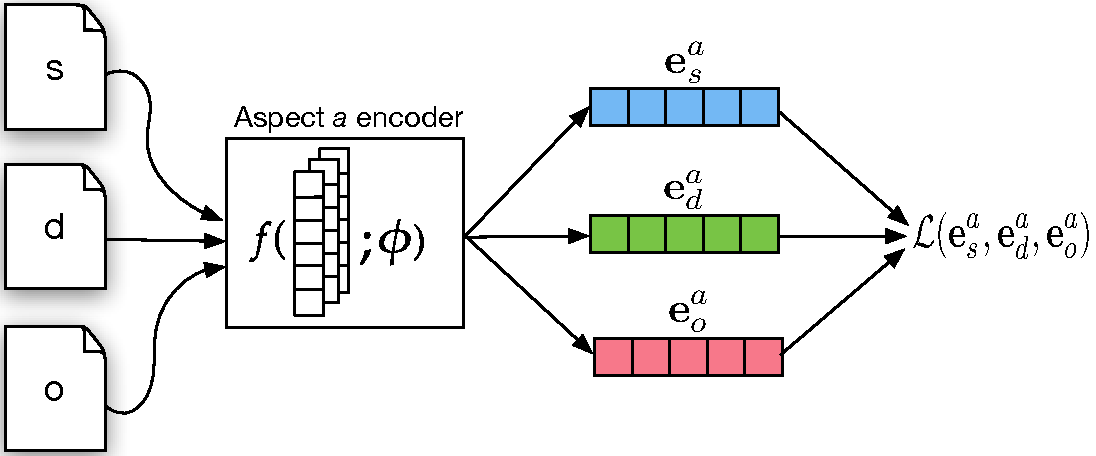
\includegraphics[width=\columnwidth]{figures/disentangle.pdf}
    \vspace{-1.5em}
    \caption{We propose associating aspects with encoders (low-level parameters are shared across aspects; this is not shown) and training these with triplets codifying aspect-wise relative similarities.}%For the specific aspect encoder architecture we use to instantiate this model in the present work, see Figure \ref{fig:encoder}.}
    \label{fig:the-idea}
    \vspace{-.75em}
\end{figure}




 %to induce our aspect-specific distributed representations; we next describe the model for this used in the present work.%, and a loss function that instantiates the above objective.

%\subsection{Exploiting Direct Triplet Supervision}
%\label{section:objective}



%\noindent The documents may or may not be drawn from the same population. For example, in one case we consider (the PICO data), we use  explicit aspect-specific summaries for $d^0$ and $d^2$. Regardless, the aim is to use this supervision to train models to induce disentangled, aspect-specific embeddings from input texts, i.e., $\mathbf{e^a_d}$ for any given document $d$ and aspect $a$. By \emph{disentangled}, we mean that this distributed representation should capture all information relevant to aspect $a$, and only this information. 
% bcw: maybe discuss here (as we did in NSF proposal) about explicit segmentation vs. non-segmentation approaches
% sarthak: Also some more explanation on PICO framework, since that was a problem in original paper
% bcw; this is now in the above

%The preceding describes the simplest scenario we consider, in which we aim to induce representations of unstructured aspects. In certain cases, however, aspects may exhibit hierarchical structure, as in the case of aspect-specific sentiment. In this case we have nested aspects, $\mathcal{A} \times \mathcal{S}$, and our supervision signal may be in some sense confounded by triplets that measure similarity with respect to pairs of these aspects. Again, an intuitive example of this is with aspect-specific sentiment: we can induce from such ratings implicit joint aspect-sentiment similarities, but we would like to tease apart the sentiment component from the aspects. 

%\section{Related Work}

%\section{Task Formulation}

%We now concretely define the problem we set out to address. Consider a set of documents D = $\{D_i\}_{i=1}^{|D|}$ where each document is composed of a sequence of $n$ words $(w_{i1}, ..., w_{in})$. In this work we assume that there exist $r$ latent salient aspects $\mathcal{A} = \{a_1, ..., a_r\}$ for which we might induce corresponding, distinct distributed representations. Formally, we aim to generate for each document $D_i$ a set of document embeddings {\boldmath$\{e^1_{i}, ..., e^r_{i}\}$}, such that each embedding $\mathbf{e^j_{i}}$ contains information pertaining to aspect $a_j$ only. We consider such embeddings \textit{disentangled}.

%sarthak : The paragraph above seems a bit qualitative. We need to define what we mean by aspects really (but then again thats our point isn't it, that we may not be able to define aspects quantitatively, but only in terms of similarity pairs). Thus it is something like learning by examples.

%Our view is that attempting to uncover such aspect-specific representations in the absence of any supervision (i.e., in a completely unsupervised setting) is likely not meaningful. Therefore, we consider weakly supervised scenarios. More specifically, we consider two concrete training settings to achieve this goal. 


%Note that for a given document, there may be multiple ways to define a set of abstracts and a completely unsupervised approach like Topic Modeling may generate a set not corresponding to user's requirements. 

%sarthak : Might be interesting to talk about supervised LDA or Labeled LDA.
% bcw: agree -- though sLDA requires a type of supervision that we are not (yet) assuming access to



%In the first, we assume a relatively strong form of supervision: aspect-specific free-text summaries matched to documents. Concretely, in this setting we assume that for each document $D_i$, we have a set of summaries $S_i = \{s_{i1}, ..., s_{ir}\}$ where each summary provides the information about the corresponding aspect $a_i$ present in $D_i$. This setting is motivated by our real-world application, in which we have access to biomedical abstracts describing clinical trials matched with free-text summaries of clinically salient aspects (see Section XX). 

%In the second setting, we aim to relax the requisite supervision, and thereby generalize our approach. We assume access to training data in the form of aspect-specific triplets $\{(D_0, D_s, D_d; a)\}$, where each such triplet implies that document $D_0$ is more similar to document $D_s$ than document $D_d$ with respect to aspect $a$. Succinctly, denoting by $\text{sim}_a$ a function codifying similarity between two its two arguments (documents) in terms of aspect $a \in \mathcal{A}$: 




% bcw: suggest having 1 para on general enc/dec approach (independent of, e.g., convnet vs other architecture) then one on our specific architecture, emphasis on adversarial thing + picture. 

%At a high level, our models are instantiations of the general encoder-decoder framework \cite{}. ...
%At a high level, our model consist of a set of encoders $\{enc_a\}$ that maps a document $d \in D$ to an aspect embedding $\mathbf{e^a_d} \in R^n$. These embeddings are trained using following training regimes :

%For each summary $s_{ij}$ in $S_i$, we construct a triplet as follows : $(D_i, s_{ij}, s_{kj})$ where $s_{kj}$ is the $j^{th}$ aspect summary for some other document $D_k$. Once the triplets are constructed, we proceed as below.

%sarthak : PROBLEM !!! No disentanglement using this (need to explicitly generate triplet (d_i, s_ij, s_ik) for disentanglement. Kind of explicitly telling the model focus on this and not focus on that.
% bcw: right agree -- need to have both terms in the objective. again would view this as first disentangling, and then differentiating within aspects. 

%\subsection{Triplet Based Training}

%Under triplet regime, each input to the model is represented as a triplet $(D_0, D_s, D_d; a)$. 



% bcw: will need to make sure we're consistent w/notation -- e.g., bolding of vectors or not, and also need to make sure this is consistent w/figures.
% bcw: suggest that we use U pper case (non-bold) for matrix / tensor, bolded lower case for vector and lowercase (non-bold) for scalar. i don't feel strongly about this but we do need to be consistent.

% bcw 5/18 -- amusingly we are ourselves guilty of talking about explainability without being precise about what sort (as per the other paper)
\vspace{-.25em}
\subsection{Encoder Architecture}
\label{section:encoder}
\vspace{-.25em}

Designing an aspect-based model requires specifying an encoder architecture. One consideration here is interpretability: a desirable property for aspect encoders is the ability to identify salient words for a given aspect. With this in mind, we propose using gated CNNs, which afford introspection via the token-wise gate activations. 

% bcw: to clarify -- H_l is indeed a matrix now?
% bcw 2/19: schematizes is too a word, overleaf!!
Figure \ref{fig:encoder} schematizes our encoder architecture. The input is a sequence of word indices $d = (w_{1}, ..., w_{N})$ which are mapped to $m$-dimensional word embeddings and stacked into a matrix $E = [{\mathbf e}_1, ..., {\mathbf e}_N]$. These are passed through sequential convolutional layers $C_1, ..., C_L$, which induce representations $H_l \in \mathbb{R}^{N \times k}$:

\vspace{-.5em}
\begin{equation}
\vspace{-.2em}
H_l = f_e(X * K_l + {\mathbf b_l})
%\vspace{-.1em}
\end{equation}

\noindent where $X \in \mathbb{R}^{N \times k}$ is the input to layer $C_l$ (either a set of $n$-gram embeddings or $H_{l-1}$) and $k$ is the number of feature maps. Kernel $K_l \in \mathbb{R}^{F \times k \times k}$ and ${\mathbf b_l} \in \mathbb{R}^{k}$ are parameters to be estimated, where $F$ is the size of kernel window.\footnote{The input to $C_1$ is $E \in \mathbb{R}^{N \times m}$, thus $K_1 \in \mathbb{R}^{F \times m \times k}$.} An activation function $f_e$ is applied element-wise to the output of the convolution operations. We fix the size of $H_{l-1} \in \mathbb{R}^{N \times k}$ by zero-padding where necessary. Keeping the size of feature maps constant across layers allows us to introduce residual connections; the output of layer $l$ is summed with the outputs of preceding layers before being passed forward. 

\begin{figure}
	\centering
    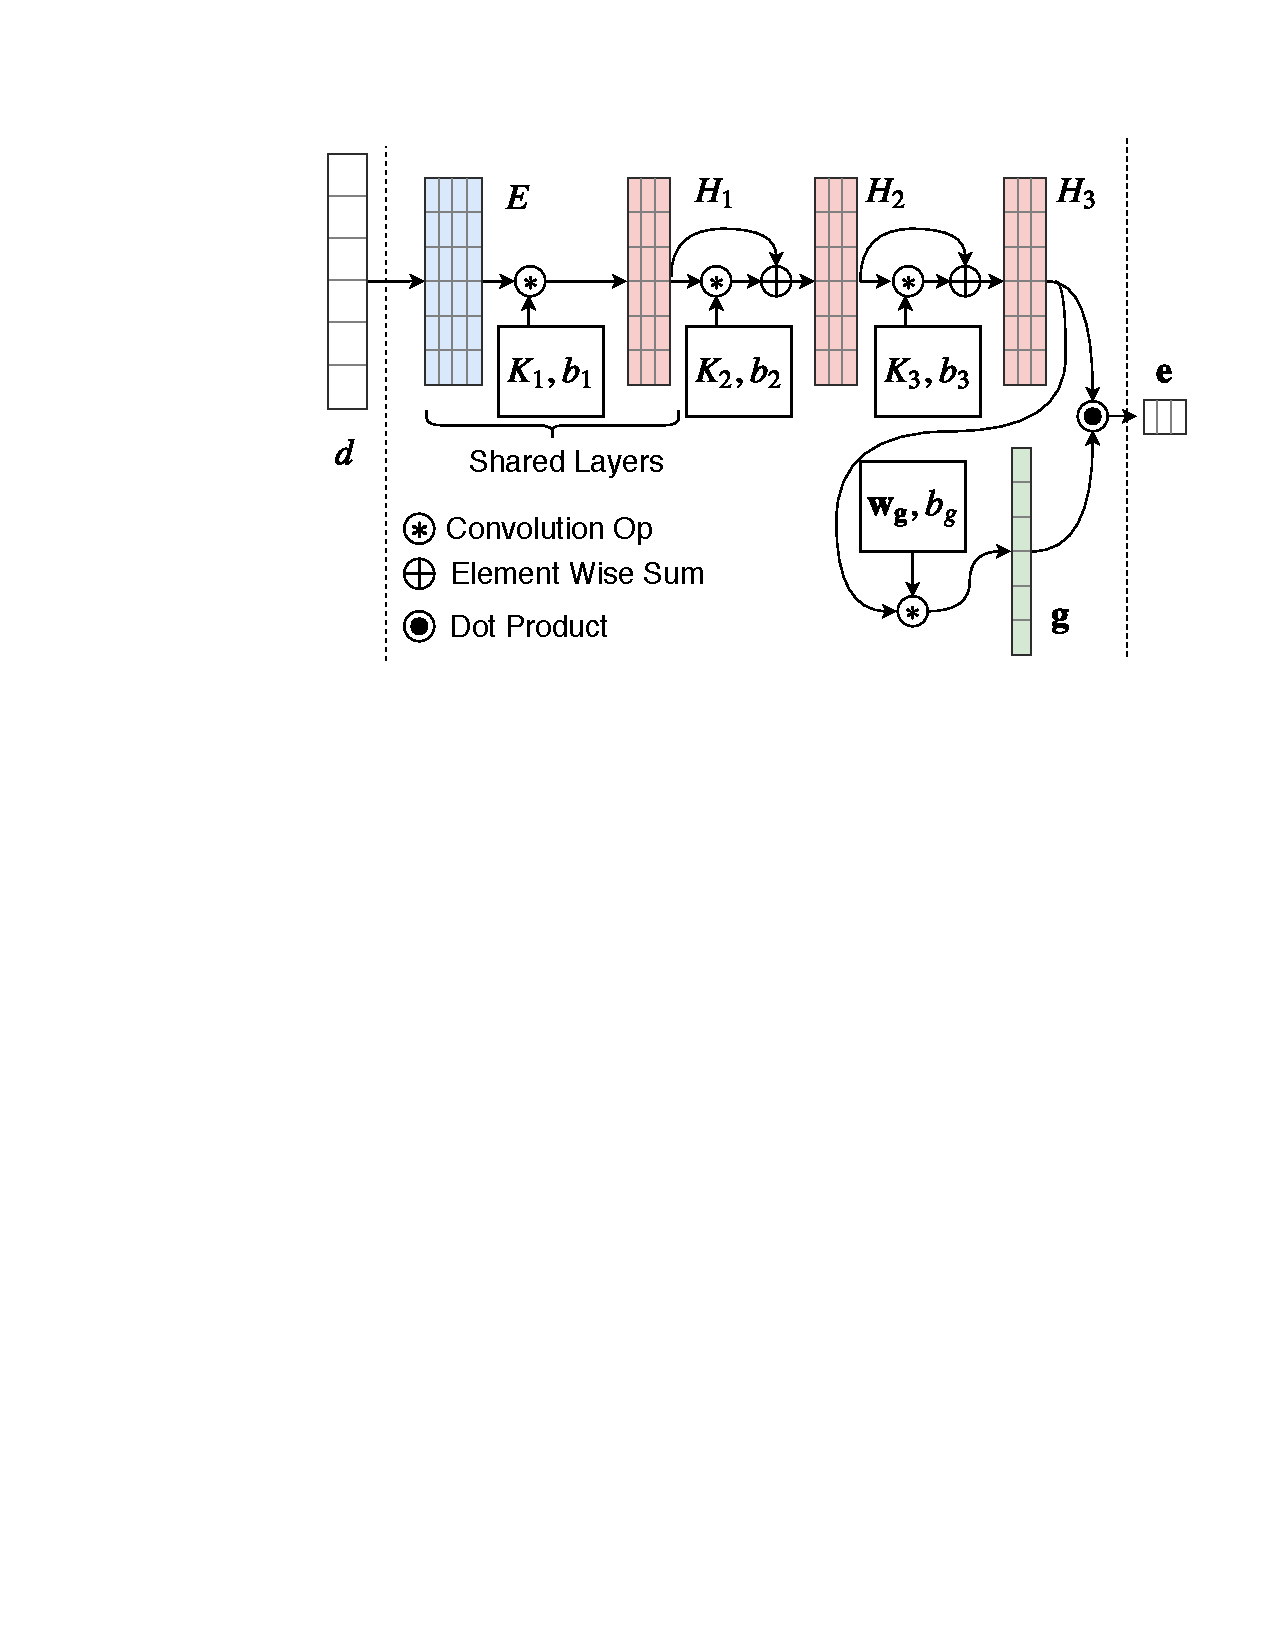
\includegraphics[width=\columnwidth]{figures/model.pdf}
     \vspace{-.75em}
    \caption{Schematic of our encoder architecture.}
    \label{fig:encoder}
    \vspace{-.65em}
\end{figure}


% bcw: changed G to lowercase and bolded, since a vector
%\par 
We multiply the output of the last convolutional layer $H_L \in \mathbb{R}^{N \times k}$ with gates ${\mathbf g} \in \mathbb{R}^{N \times 1}$ to yield our final embedding ${\mathbf e_d} \in \mathbb{R}^{1 \times k}$: %\vspace{-.1em}

% bcw: I don't think we should use K here, since this overloads that variable
\begin{equation}
%\vspace{-.35em}
\begin{aligned}
{\mathbf g} &= \sigma(H_L \cdot {\mathbf w}_g + b_g) \\
{\mathbf e_d} &= {\mathbf g}^T H_L
\end{aligned}
%\vspace{-.1em}
\label{eq:gate}
\end{equation}




\noindent where ${\mathbf w}_g \in \mathbb{R}^{k \times 1}$ and $b_g \in \mathbb{R}$ are learned parameters and $\sigma$ is the sigmoid activation function. We impose a sparsity-inducing constraint on $\mathbf{g}$ via the $\ell_1$ norm; this allows the gates to effectively serve as an attention mechanism over the input. Additionally, to capture potential cross-aspect correlation, weights in the embedding and first convolutional layers are shared between aspect encoders. 
%weights of embedding layer and first convolutional layer are shared between aspects.


%Effectively, the gates act as an attention mechanism if we impose . Thus, our loss function takes an additional term of form $||G||$.

%sarthak : Is time dimension right phrase to use ?
% bcw: i wouldn't say it's *wrong* but would prefer to avoid just because it might confuse some people -- maybe stick with rows or over words or tokens or whatever
% Finally, we sum over the rows of $H'_L \in R^{N \times k}$ to induce our final embedding $\mathbf{e}_d \in R^{k}$. % The architecture is depicted in Figure \ref{fig:encoder}. % bcw: already say this above

%\subsubsection{Other variants}
\vspace{.2em}
\noindent {\bf Alternative encoders}. To assess the relative importance of the specific encoder model architecture used, we conduct experiments in which we fine-tune standard document representation models via triplet-based training. Specifically, we consider a single-layer MLP with BoW inputs, and a Neural Variational Document Model (NVDM) \cite{miao2016neural}. For the NVDM we take a weighted sum of the original loss function and the triplet-loss over the learned embeddings, where the weight is a model hyperparameter.
%sarthak : We may include sparsity for this.

%sarthak : Want to say Disentanglement depends on correlation between aspects. If correlation high, difficult to marginalize over other aspects since model will be confused over what to differentiate on. 

%sarthak : Thats why we need the second set of triplets (d_i, s_ij, s_ik) in PICO case.

%\vspace{-.45em}
\section{Varieties of Supervision}
%\vspace{-.5em}
Our approach entails learning from triplets that codify relative similarity judgments with respect to specific aspects. We consider two approaches to acquiring such triplets: the first exploits aspect-specific summaries written for texts, and the second assumes a more general scenario in which we solicit aspect-wise triplet judgments directly.

%\vspace{-.5em}
\subsection{Deriving Triplets from Aspect Summaries}
%\vspace{-.5em}
% % bcw: a stylistic thing (admittedly subjective): i suggest avoiding 'Let the ...' or 'Let us... ', because it reads a bit too didactic in tone for a conference paper (more appropriate for a textbook i think).
% % bcw: also, 'has' -> 'have' when the arg is plural  (e.g., 'assume the document has n words', rather than 'assume the document have n words'

%Aspect-specific summaries written for texts (documents) constitutes one potential mechanism of indirect supervision. 
In the case of our motivating example 
-- 
%learning to induce 
disentangled representations for articles describing clinical trials 
%that codify clinically relevant aspects 
-- 
we have obtained aspect-specific summaries from the \emph{Cochrane Database of Systematic Reviews (CDSR)}. Cochrane is an international organization that creates and curates biomedical \emph{systematic reviews}. Briefly, such reviews seek to formally synthesize all relevant articles to answer precise clinical questions, i.e., questions that specify a particular PICO frame. The CDSR consists of a set of reviews $\{R_i\}$. Reviews include multiple articles (studies) $\{S_{ij}\}$. Each study $S$ consists of an abstract $A$ and a set of free text summaries $(s_P, s_I, s_O)$ written by reviewers describing the respective P, I and O elements in $S$.

%The CDSR includes data from thousands of previously conducted reviews, each of which comprises multiple studies. Each study consists of an abstract along with a set of free text summaries written by reviewers describing the respective PICO elements in the study, thus yielding an indirect training signal regarding aspects. We propose to exploit this by assembling aspect triplets for abstracts.%comprising abstracts (the documents to be encoded). % and aspect-specific summaries. 
%The review process entails writing free-text summaries describing the PICO elements in each study. We can match these summaries to corresponding study abstracts.




%This data includes free-text summaries written by reviewers describing the respective PICO elements of individual studies. We can match these summaries to published abstracts,

%This provides 

% bcw 2/21 -- both the reviewer and dave have noted that this is sort of hard to follow (even re-written), and I don't disagree, but honestly this complexity may just be necessary...
%Specifically, we are to learn from article abstracts paired with aspect-specific summaries written by domain experts. 
%As mentioned above, studies in the CDSR are grouped into systematic reviews, which again implicitly specify PICO frames. 

% bcw 5/2 -- I have tried (once again!) to make this is a bit easier to follow, but still quite dense. However, I think (hope) that the first paragraph below helps a bit
Reviews implicitly specify PICO frames, and thus two studies in any given review may be viewed as equivalent with respect to their PICO aspects. We use this observation to derive document triplets. Recall that triplets for a given aspect include two comparatively similar texts ($s$, $d$) and one relatively dissimilar ($o$). Suppose the aspect of interest is the trial population. Here we match a given abstract ($d$) with its matched population summary from the CDSR ($s$); this encourages the encoder to yield similar embeddings for the abstract and the population description. The dissimilar $o$ is constructed to distinguish the given abstract from (1) other aspect encodings (of interventions, outcomes), and, (2) abstracts for trials with different populations.

Concretely, to construct a triplet  $(s, d, o)$ for the PICO data, we draw two reviews $R_1$ and $R_2$ from the CDSR at random, and sample two studies from the first ($s_1, s_1'$) and one from the second ($s_2$). Intuitively, $s_2$ will (very likely) comprise entirely different PICO elements than ($s_1, s_1'$), by virtue of belonging to a different review. To formalize the preceding description, our triplet is then: $(s = [s_1'^P], d = [s_1^{\text{abstract}}], o = [s_2^P|s_1'^I|s_1'^O])$, where $s_1^{\text{abstract}}$ is the abstract for study $s_1$, and aspect summaries for studies are denoted by superscripts. We include a concrete example of triplet construction in the Appendix, Section D.

\begin{comment}
\subsubsection{Example of PICO Triplet generation}
As an illustrative example, we walk through construction of a single triplet for the PICO domain in detail. Recall that we first randomly draw two reviews, $R_1$ and $R_2$. In this case, $R_1$ consists of studies involving nocturnal enuresis and $R_2$ concerns asthma. From $R_1$ we randomly select two studies $S, S'$. 

(1) Here we sample abstract $A$ for study $S$, shown below:

{\footnotesize \begin{quote}
In recent years the treatment of primary nocturnal enuresis (PNE) with desmopressin (DDAVP) has been promising. The route of administration until now had been intranasal, but because the tablets were introduced for the treatment of diabetes insipidus they have also become available for the treatment of PNE. \ldots The effect of oral desmopressin (1-deamino-8-D-arginine-vasopressin) (DDAVP tablets, Minirin) was investigated in 25 adolescents (ages 11 to 21 years) with severe monosymptomatic nocturnal enuresis. \ldots The final part was an open long-term study consisting of two 12-week treatment periods. The efficacy of the drug was measured in reductions of the number of wet nights per week. \ldots the number of wet nights decreased from a mean of 4.9 to 2.8. During the double-blind period, a significant reduction of wet nights was observed (1.8 vs 4.1 for placebo). \ldots After cessation of the drug, 44\% of the patients had a significant decrease in the number of wet nights. Oral desmopressin has a clinically significant effect on patients with PNE, and therapy is safe when administered as long-term treatment. \end{quote}}

For study $S$, the summaries in the CDSR are: 

\noindent \textbf{P summary $(s_P)$}

{\footnotesize \begin{quote} Number of children: 10. Inclusion criteria: adolescents (puberty stage at least 2, at least 12 years).  Exclusion criteria: treatment in previous 2 weeks, daytime wetting, UTI. Baseline wetting 4.7 (SD 1.1) wet nights/week Department of Paediatric Surgery, Sweden\end{quote}}

\noindent \textbf{I Summary $(s_I)$}
{\footnotesize \begin{quote} A : desmopressin orally (dosage based on titration period) B : placebo Duration 4 weeks each
\end{quote}}

\noindent \textbf{O summary $(s_O)$}
{\footnotesize \begin{quote} Wet nights during trial (number, mean, SD): A: 10, 1.8 (SD 1.4); B: 10, 4.1 (1.5) Side effects: headache (5); abdominal pain (6); nausea and vertigo (1) All resolved while treatment continued \end{quote}}

\vspace{-1em}
\par\noindent\rule{\columnwidth}{0.4pt}
(2) From study $S'$, the summaries in the CDSR are reproduced as follows. 

\noindent \textbf{P Summary $(s'_P)$}

{\footnotesize \begin{quote} Number of children: 135 Dropouts: 23 excluded for non-compliance, and 39 lost to follow up including 12 failed with alarms. Inclusion criteria: monosymptomatic nocturnal enuresis, age $>5$ years. \ldots\end{quote}}

\noindent \textbf{I Summary $(s'_I)$} 
{\footnotesize \begin{quote} A (62): desmopressin 20 g intranasally increasing to 40 g if response partial B (73): alarm (pad-and-bell) Duration of treatment 3 months. If failed at that time, changed to alternative arm\end{quote}}

\noindent \textbf{O summary $(s'_O)$}
{\footnotesize \begin{quote} DRY nights at 3 months: A 85\%; B: 90\% Number not achieving 14 dry nights: A 12/39; B: 6/37 Side effects: not mentioned \end{quote}}

% \vspace{1em}
\vspace{-1em}
\par\noindent\rule{\columnwidth}{0.4pt}
(3) From review $R_2$, we sample one study $S''$. Matched summaries in the CDSR are as follows. 

\noindent \textbf{P Summary $(s''_P)$}

{\footnotesize \begin{quote} n = 8, Mean age = 52, Inclusion: intrinsic asthma, constant reversibility $>$ 20\% None had an acute exacerbation at time of study Exclusion: none listed \end{quote}}

\noindent \textbf{I summary $(s''_I)$}

{\footnotesize \begin{quote} \#1: Atenolol 100 mg Metoprolol 100 mg Placebo \#2: Terbutaline (IV then inhaled) after Tx or placebo \end{quote}}

\noindent \textbf{O summary $(s''_O)$}

{\footnotesize \begin{quote} FEV1 Symptoms \end{quote}}

% \vspace{1em}
\vspace{-1em}
\par\noindent\rule{\columnwidth}{0.4pt}
(4) We note how the summaries for $S$ and $S'$ are similar to each other (but not identical) since they belong in the same review whereas they are quite different from summaries for $S''$ which belongs in a different review. Now we construct the triplet $(s, d, o)_P$ as follows:

% \vspace{1em}
\noindent {\boldmath $s = s'_P$}:

{\footnotesize \begin{quote} Number of children: 135 Dropouts: 23 excluded for non-compliance, and 39 lost to follow up including 12 failed with alarms Inclusion criteria: monosymptomatic nocturnal enuresis, age $>5$ years Exclusion criteria: previous treatment with DDAVP or alarm, urological pathology, diurnal enuresis, UTI Age, mean years: 11.2  Baseline wetting: A 21\% dry nights, B 14\% dry nights\end{quote}}

\noindent So we have {\boldmath $d$} \textbf{: A} and {\boldmath $o = [s''_P|s'_I|s'_O]$}: 

{\footnotesize \begin{quote} n = 8 Mean age = 52 Inclusion: intrinsic asthma, constant reversibility $>$ 20\% None had an acute exacerbation at time of study Exclusion: none listed $|$ A (62): desmopressin 20 g intranasally increasing to 40 g if response partial B (73): alarm (pad-and-bell) Duration of treatment 3 months. If failed at that time, changed to alternative arm $|$ DRY nights at 3 months: A 85\%; B: 90\% Number not achieving 14 dry nights: A 12/39; B: 6/37 Side effects: not mentioned \end{quote}}


%Formally, to construct a triplet for aspect $a$, we randomly select two reviews and sample one study 

% From review $R_1$, we sample two studies $S, S'$ and from $R_2$, we sample one study $S''$. Let $A$ be the abstract for study $S$, $(s'_P, s'_I, s'_O)$ be the P, I and O summaries, respectively, corresponding to study $S'$, and let $s''_P$ be the population summary for $S''$. We assemble these into a triplet $(s, d, o) = (s = [s'_P], d = A, o = [s''_P|s'_I|s'_O])$ where $o$ is constructed by concatenating $s''_P$ with $s'_I$ and $s'_O$. Thus, using this triplet, our model learns to distinguish study $d$ on the basis of aspect $a$, even if the $o$ document contains the same information as $d$ for all other aspects. We include a concrete example of triplet construction in the Appendix, Section D.

%  Specifically, we adopt a variant of adversarial training. T

%we start with a randomly sampled study abstract $d$, belonging to review $R$ in the CDSR. We sample summaries $\{s_k\}$ for all aspects $k$ written for a different study $d'$ included in the same review $R$. We then sample a summary $o_a$ which describes aspect $a$ of a study $d''$ from a \emph{different} systematic review $R'$ than the one to which $d, d'$ belongs.\footnote{By virtue of belonging to a different review, it is likely, though not certain, that the study PICO elements will differ.} We assemble these in triplet $(s, d, o)_a = (s = [s_a], d = d, o = [o_a|\{s_{a'}\}])$ where $o$ is constructed by concatenating $o_a$ with all summaries $\{s_{a'}\}$ such that $a' \neq a$. Thus, under this triplet, our model learns to distinguish documents $d$ on the basis of aspect $a$ even if the $o$ document contains the same information as $d$ for all other aspects $a'$.




% To ensure that representations are aspect-specific, we assemble a second triplet type $(s, d, o)^2_a$ wherein $o$ is sampled from summaries in the same review $R$ but describing a \emph{different} aspect $a'$ while $s$ is reused from above. In this scenario, we use separate encoder model instantiations (that is, parameterized independently).


% Because these summaries were written by different people (working with different teams), they vary substantially in many respects, including length, structure and grammar. Nonetheless they contain valuable signal regarding aspects that we aim to exploit by assembling triplets comprising biomedical abstracts (the documents to be encoded) and matched aspect-specific summaries. 


%we aim to find functions $f_A: \mathcal{A} \rightarrow \mathbb{R}^d$ and $f_P: \mathcal{P} \rightarrow \mathbb{R}^d$ such that $\texttt{sim}(f_A(a), f_S(p)) \triangleq s$ is large, under similarity metric $\texttt{sim}$. Here $\mathcal{A}$ denotes the space of clinical abstract texts, $\mathcal{P}$ the space of all population summaries, and $d \in \mathbb{N}+$ is a hyperparameter. To reduce overfitting, we rely on adversarial training; specifically we sample `imposter' example summaries $\tilde{p}$ which describe the population of a trial from a \emph{different} systematic review.\footnote{By virtue of belonging to a different review, it is likely (though not certain) that the trial populations will differ.}
%We have such summaries in the case of our motivating application: abstracts of articles that describe randomized controlled trials (RCTs). Specifically, we have access to the \emph{Cochrane Database of Systematic Reviews (CDSR)}, which comprises abstractive summaries manually written for articles describing clinical trials that included in biomedical systematic reviews (or, "meta-analyses"). This follows the paradigm of Evidence-Based Medicine (EBM), wherein it is customary to formulate answerable, precise clinical questions with respect to trial Populations, Interventions, Comparators and Outcomes of interest. Collectively, these aspects are referred to as PICO \cite{sackett1996evidence}. Because the distinction between interventions and comparators is arbitrary, the intervention and comparator aspects may be collapsed into a single I/C aspect.


%Formally, we assume a given document $d$ comes attached with a set of $r$ aspect summaries $S^d = \{s^d_1, ..., s^d_r\}$. For each aspect $j$, 

%\begin{comment}
To realize this we adopt a distantly supervised training paradigm in which we assume access to aspect specific free-text summaries for a set of corresponding documents. Here we obtained such data from the \emph{Cochrane Database of Systematic reviews (CDSR)}. Cochrane is an international organization that promotes and assists with the creation and curation of \emph{systematic reviews}, which underpin EBM. Briefly, systematic reviews seek to answer precise clinical questions; that is, questions that specify a particular PICO frame (Table \ref{table:pico-framework}). Such reviews therefore provide a natural source of training and testing data for our proposed approach.

The CDSR includes the data generated for thousands of previously conducted systematic reviews, which each in turn comprise multiple studies. Part of the review process entails writing free-text summaries describing the PICO elements studied in each constituent trial. These summaries are stored in the CDSR, and we can match them to corresponding abstracts. Because these summaries were written by different people (working with different teams), they vary greatly in many respects, including length, structure and grammar. 
%\subsection{Learning Objective}

Given an abstract $a$ and summary of the population aspect (we outline the learning objective for P embeddings; procedures for I/C and O embeddings are analogous) $p$ for $a$, we aim to find functions $f_A: \mathcal{A} \rightarrow \mathbb{R}^d$ and $f_P: \mathcal{P} \rightarrow \mathbb{R}^d$ such that $\texttt{sim}(f_A(a), f_S(p)) \triangleq s$ is large, under similarity metric $\texttt{sim}$. Here $\mathcal{A}$ denotes the space of clinical abstract texts, $\mathcal{P}$ the space of all population summaries, and $d \in \mathbb{N}+$ is a hyperparameter. To reduce overfitting, we rely on adversarial training; specifically we sample `imposter' example summaries $\tilde{p}$ which describe the population of a trial from a \emph{different} systematic review.\footnote{By virtue of belonging to a different review, it is likely (though not certain) that the trial populations will differ.}
\end{comment}


% we construct a similar pseudo-document $D_s$ by concatenating the aspect j summary of document i with corrupt summaries for all other aspects.

% bcw : we do not do this actually, right? 
% sarthak : No we don't.
% Thus, $D_s$ has same value for aspect j and some negative value for all other aspects. Similarly, we construct a negative pseudo-document $D_d$ by concatenating a negative summary for aspect j and a same summaries for all other aspect as $D_i$. The triplet $(D_i, D_s, D_d; j)$ then form a training point for aspect $j$ used as above. 

%\vspace{-.25em}
% \end{comment}

\subsection{Learning Directly from Aspect-Wise Similarity Judgments}
%\vspace{-.25em}
The preceding setup assumes a somewhat unique case in which we have access to aspect-specific summaries written for texts. As a more general setting, we also consider learning directly from triplet-wise supervision concerning relative similarity with respect to particular aspects \cite{amid2015multiview,veit2017conditional,wilber2014cost}. The assumption is that such judgments can be solicited directly from annotators, and thus the approach may be applied to arbitrary domains, so long as meaningful aspects can be defined implicitly via pairwise similarities regarding them. 

We do not currently have corpora with such judgments in NLP, so we constructed two datasets using aspect-specific sentiment ratings. Note that this highlights the flexibility of exploiting aspect-wise triplet supervision as a means of learning disentangled representations: existing annotations can often be repurposed into such triplets. 

% bcw: TODO elaborate ... 

%% bcw: something about how this is what vision people do. also, should cite literature about how people can totally make these kinds of judgments




%\vspace{-.5em}
\section{Datasets and Experiments}
%\vspace{-.5em}
\label{section:experiments}

% bcw 2/19 -- i think we might want to move the table up a page.
% \begin{table*}%[!htb]
% \small
% \centering
% \begin{tabular}{l r r r r r|r r || r r r r}
% \hline
% Method &  TF-IDF &  Doc2Vec&  LDA &  NVDM &  ABAE&  RR-TF &  DSSM & $\mathbf{P}$ & $\mathbf{I}$ & $\mathbf{O}$ & $\mathbf{[P|I|O]}$ \\ 
% \hline
% % ACEInhib.  & 0.81 & 0.74 & 0.72 & 0.85 & 0.81 & 0.67 & 0.85 & 0.83 & 0.88 & 0.84 &  \textbf{0.92} \\
% % ADHD  & 0.90 & 0.82 & 0.83 &  \textbf{0.93}  & 0.77 & 0.85 & 0.83 & 0.86 & 0.75 & 0.91 &  0.89 \\ 
% % Antihist. & 0.81 & 0.73 & 0.67 & 0.79 & 0.84 & 0.72 & \textbf{0.91} & 0.88 & 0.84 & 0.89 &  \textbf{0.91} \\  
% % Antipsych.  & 0.75 & 0.85 & 0.88 & 0.89 & 0.81 & 0.63 & 0.96 & 0.91 & 0.93 &  \textbf{0.97} &  \textbf{0.97} \\ 
% % BetaBlockers  & 0.67 & 0.65 & 0.61 & 0.76 & 0.70 & 0.56 & 0.68 & 0.71 & 0.75 & 0.77 &  \textbf{0.81} \\ 
% % CCBlockers  & 0.67 & 0.60 & 0.67 & 0.70 & 0.69 & 0.58 & 0.76 & 0.73 & 0.69 & 0.74 &  \textbf{0.77} \\ 
% % Estrogens  & 0.87 & 0.85 & 0.60 & 0.94 & 0.85 & 0.82 & 0.96 &  \textbf{1.00} & 0.98 & 0.83 &  \textbf{1.00} \\ 
% % NSAIDS  & 0.85 & 0.77 & 0.73 & 0.9 & 0.77 & 0.74 & 0.89 & 0.94 &  \textbf{0.95} & 0.8 &  \textbf{0.95} \\ 
% % Opiods  & 0.81 & 0.75 & 0.80 & 0.83 & 0.77 & 0.76 & 0.86 & 0.80 & 0.83 &  \textbf{0.92} &  \textbf{0.92} \\ 
% % OHG  & 0.79 & 0.80 & 0.70 & 0.89 & 0.90 & 0.72 & 0.90 & 0.90 & 0.95 & 0.95 &  \textbf{0.96} \\
% % PPI  & 0.81 & 0.79 & 0.74 & 0.85 & 0.82 & 0.68 & 0.94 & 0.94 & 0.87 & 0.87 &  \textbf{0.95} \\  
% % MuscleRelax.  & 0.60 & 0.67 & 0.74 & 0.75 & 0.61 & 0.57 & 0.77 & 0.68 & 0.62 &  \textbf{0.78}&  0.75 \\ 
% % Statins  & 0.79 & 0.76 & 0.66 & 0.87 & 0.77 & 0.68 & 0.87 & 0.82 &  \textbf{0.94} & 0.87 &  \textbf{0.94} \\  
% % Triptans  & 0.92 & 0.82 & 0.83 & 0.92 & 0.75 & 0.81 & \textbf{0.97}& 0.93 & 0.79 &  \textbf{0.97}  &  \textbf{0.97} \\  
% AUC & 0.79 & 	0.76 & 	0.73 & 	0.85 & 	0.78 & 	0.70 & 	0.87 & 	0.85 & 	0.84 & 	0.87 & 	\textbf{0.91}
% \end{tabular}
% \vspace{-.65em}
% \caption{Mean AUCs achieved using different representations over the \newcite{cohen2006reducing} corpus. Models to the right of the $\vert$ are supervised; those to the right of $\vert \vert$ use the proposed disentangled embeddings. } 
% %\vspace{-1em}
% \label{table:cohenauc}
% \end{table*}

\begin{table*}%[!htb]
\small
\setlength{\tabcolsep}{3pt}
\centering
\begin{tabular}{l r r r r r|r r || r r r r}
Study &  TF-IDF &  Doc2Vec&  LDA &  NVDM &  ABAE&  RR-TF &  DSSM & $\mathbf{P}$ & $\mathbf{I}$ & $\mathbf{O}$ & $\mathbf{[P|I|O]}$ \\ 
\hline
ACEInhib.  & 0.81 & 0.74 & 0.72 & 0.85 & 0.81 & 0.67 & 0.85 & 0.83 & 0.88 & 0.84 &  \textbf{0.92} \\
ADHD  & 0.90 & 0.82 & 0.83 &  \textbf{0.93}  & 0.77 & 0.85 & 0.83 & 0.86 & 0.75 & 0.91 &  0.89 \\ 
Antihist. & 0.81 & 0.73 & 0.67 & 0.79 & 0.84 & 0.72 & \textbf{0.91} & 0.88 & 0.84 & 0.89 &  \textbf{0.91} \\  
Antipsych.  & 0.75 & 0.85 & 0.88 & 0.89 & 0.81 & 0.63 & 0.96 & 0.91 & 0.93 &  \textbf{0.97} &  \textbf{0.97} \\ 
BetaBlockers  & 0.67 & 0.65 & 0.61 & 0.76 & 0.70 & 0.56 & 0.68 & 0.71 & 0.75 & 0.77 &  \textbf{0.81} \\ 
CCBlockers  & 0.67 & 0.60 & 0.67 & 0.70 & 0.69 & 0.58 & 0.76 & 0.73 & 0.69 & 0.74 &  \textbf{0.77} \\ 
Estrogens  & 0.87 & 0.85 & 0.60 & 0.94 & 0.85 & 0.82 & 0.96 &  \textbf{1.00} & 0.98 & 0.83 &  \textbf{1.00} \\ 
NSAIDS  & 0.85 & 0.77 & 0.73 & 0.9 & 0.77 & 0.74 & 0.89 & 0.94 &  \textbf{0.95} & 0.8 &  \textbf{0.95} \\ 
Opioids  & 0.81 & 0.75 & 0.80 & 0.83 & 0.77 & 0.76 & 0.86 & 0.80 & 0.83 &  \textbf{0.92} &  \textbf{0.92} \\ 
OHG  & 0.79 & 0.80 & 0.70 & 0.89 & 0.90 & 0.72 & 0.90 & 0.90 & 0.95 & 0.95 &  \textbf{0.96} \\
PPI  & 0.81 & 0.79 & 0.74 & 0.85 & 0.82 & 0.68 & 0.94 & 0.94 & 0.87 & 0.87 &  \textbf{0.95} \\  
MuscleRelax.  & 0.60 & 0.67 & 0.74 & 0.75 & 0.61 & 0.57 & 0.77 & 0.68 & 0.62 &  \textbf{0.78}&  0.75 \\ 
Statins  & 0.79 & 0.76 & 0.66 & 0.87 & 0.77 & 0.68 & 0.87 & 0.82 &  \textbf{0.94} & 0.87 &  \textbf{0.94} \\  
Triptans  & 0.92 & 0.82 & 0.83 & 0.92 & 0.75 & 0.81 & \textbf{0.97}& 0.93 & 0.79 &  \textbf{0.97}  &  \textbf{0.97} \\  \hline
Mean & 0.79	& 0.76& 	0.73& 	0.85& 	0.78& 	0.70& 	0.87& 	0.85& 	0.84& 	0.87& 	\textbf{0.91}
\end{tabular}
\vspace{-.65em}
\caption{AUCs achieved using different representations on the Cohen et al. corpus. Models to the right of the $\vert$ are supervised; those to the right of $\vert \vert$ constitute the proposed disentangled embeddings. } 
%\vspace{-1em}
\label{table:cohenauc}
\end{table*}


We present a series of experiments on three corpora to assess the degree to which the learned representations are disentangled, and to evaluate the utility of these embeddings in simple downstream retrieval tasks. We are particularly interested in the ability to identify documents similar w.r.t.~a target aspect. All parameter settings for baselines are reported in the Appendix (along with additional experimental results), and all code will be made available upon publication.
%In this section, we present the experimental results on 3 datasets to validate our proposed approach.

%\vspace{-.5em}
\subsection{PICO (EBM) Domain}
\label{section:PICO}
\vspace{-.25em}

We first evaluate embeddings quantitatively with respect to retrieval performance. In particular, we assess whether the induced representations afford improved retrieval of abstracts relevant to a particular systematic review \cite{cohen2006reducing,wallace2010semi}. We then perform two evaluations that explicitly assess the degree of disentanglement realized by the learned embeddings.

The PICO dataset comprises 41K abstracts of articles describing clinical trials extracted from the CDSR. Each abstract is associated with a review and three summaries, one per aspect (P/I/O). We keep all words that occur in $\geq$ 5 documents, converting all others to $\texttt{unk}$. We truncate documents to a fixed length (set to the 95th percentile). 


%we first assess whether the induced embeddings afford better

%\par
%\noindent \textbf{Training Setup} 

\vspace{-.1em}
\subsubsection{Quantitative Evaluation}
\vspace{-.25em}

\noindent \textbf{Baselines}. We compare the proposed {\bf P}, {\bf I} and {\bf O} embeddings and their concatenation $\mathbf{[P|I|O]}$ to the following. {\bf TF-IDF}: standard TF-IDF representation of abstracts. {\bf RR-TF}: concatenated TF-IDF vectors of sentences predicted to describe the respective PICO elements, i.e., sentence predictions made using the pre-trained model from \cite{wallace2016extracting} --- this model was trained using distant supervision derived from the CDSR. {\bf doc2vec}: standard (entangled) distributed representations of abstracts \cite{le2014distributed}. {\bf LDA}: Latent Dirichlet Allocation. {\bf NVDM}: A generative model of text where the representation is a vector of log-frequencies that encode a topic \cite{miao2016neural}. {\bf ABAE}: An autoencoder model that discovers latent aspects in sentences \cite{he-2017}. We obtain document embeddings by summing over constituent sentence embeddings. {\bf DSSM}: A CNN based encoder trained with triplet loss over abstracts \cite{shen2014latent}.

\vspace{.15em}
\noindent \textbf{Hyperparameters and Settings}. We use three layers for our CNN-based encoder (with 200 filters in each layer; window size of 5) and the PReLU activation function \cite{he2015delving} as $f_e$. We use 200d word embeddings, initialized via pretraining over a corpus of PubMed abstracts \cite{moen2013distributional}. We used the Adam optimization function with default parameters \cite{kingma2014adam}. We imposed $\ell_2$ regularization over all parameters, the value of which was selected from the range ($1e$-$2$, $1e$-$6$) as $1e$-$5$. The $\ell_1$ regularization parameter for gates was chosen from the range ($1e$-$2$, $1e$-$8$) as $1e$-$6$. All model hyperparameters for our models and baselines were chosen via line search over a 10\% validation set.

\vspace{.15em}
\noindent \textbf{Metric}. For this evaluation, we used a held out set of 15 systematic reviews (comprising 2,223 studies) compiled by \newcite{cohen2006reducing}. The idea is that good representations should map abstracts in the same review (which describe studies with the same PICO frame) relatively near to one another. To compute AUCs over reviews, we first calculate all pairwise study similarities (i.e., over all studies in the Cohen corpus). We can then construct an ROC for a given abstract $a$ from a particular review to calculate its AUC: this measures the probability that a study drawn from the same review will be nearer to $a$ than a study from a different review. A summary AUC for a review is taken as the mean of the study AUCs in that review.
%a summary AUC for a given review by averaging the area under the ROC curves for each abstract $a$ that it contains 


%which  %This measures the  
%abstract in a particular review; we average the area underneath these for each abstract in a review, and t

%$A$ such that $A_{ij} = {\textit sim}(a_i, a_j)$ for abstracts $a_i$ and $a_j$ ($A_{ii}$ is set to $-\infty$). Given $A$ and a systematic review $\mathcal{R}^{(i)}$, we compute an ROC curve for each $a \in \mathcal{R}^{(i)}$ and then average these within reviews to derive a summary ROC curve for each review. 



\vspace{.15em}
\noindent \textbf{Results}. Table \ref{table:cohenauc} reports the mean AUCs over individual reviews in the \newcite{cohen2006reducing} corpus, and grand means over these (bottom row). %We report detailed results (on each individual review) in the Appendix. 
In brief: The proposed PICO embeddings (concatenated) obtain an equivalent or higher AUC than baseline strategies on 12/14 reviews, and strictly higher AUCs in 11/14. It is unsurprising that we outperform unsupervised approaches, but we also best RR-TF, which was trained with the same CDSR corpus \cite{wallace2016extracting}, and DSSM \cite{shen2014latent}, which exploits the same triplet loss as our model. We outperform the latter by an average performance gain of 4 points AUC (significant at 95\% level using independent 2-sample t-test).

\begin{table}
\small
    \centering
    \begin{tabularx}{\columnwidth}{X}
         {\setlength{\fboxsep}{0pt}\colorbox{red!16!white}{\strut in}}
{\setlength{\fboxsep}{0pt}\colorbox{red!22!white}{\strut a}}
{\setlength{\fboxsep}{0pt}\colorbox{red!24!white}{\strut clinical}}
{\setlength{\fboxsep}{0pt}\colorbox{red!13!white}{\strut trial}}
{\setlength{\fboxsep}{0pt}\colorbox{red!12!white}{\strut mainly}}
{\setlength{\fboxsep}{0pt}\colorbox{red!18!white}{\strut involving}}
{\setlength{\fboxsep}{0pt}\colorbox{red!23!white}{\strut patients}}
{\setlength{\fboxsep}{0pt}\colorbox{red!49!white}{\strut over}}
{\setlength{\fboxsep}{0pt}\colorbox{red!80!white}{\strut qqq}}
{\setlength{\fboxsep}{0pt}\colorbox{red!100!white}{\strut with}}
{\setlength{\fboxsep}{0pt}\colorbox{red!77!white}{\strut coronary}}
{\setlength{\fboxsep}{0pt}\colorbox{red!74!white}{\strut heart}}
{\setlength{\fboxsep}{0pt}\colorbox{red!82!white}{\strut disease}}
{\setlength{\fboxsep}{0pt}\colorbox{red!82!white}{\strut ,}}
{\setlength{\fboxsep}{0pt}\colorbox{red!47!white}{\strut ramipril}}
{\setlength{\fboxsep}{0pt}\colorbox{red!9!white}{\strut reduced}}
{\setlength{\fboxsep}{0pt}\colorbox{red!0!white}{\strut mortality}}
{\setlength{\fboxsep}{0pt}\colorbox{red!0!white}{\strut while}}
{\setlength{\fboxsep}{0pt}\colorbox{red!0!white}{\strut vitamin}}
{\setlength{\fboxsep}{0pt}\colorbox{red!0!white}{\strut e}}
{\setlength{\fboxsep}{0pt}\colorbox{red!0!white}{\strut had}}
{\setlength{\fboxsep}{0pt}\colorbox{red!10!white}{\strut no}}
{\setlength{\fboxsep}{0pt}\colorbox{red!10!white}{\strut preventive}}
{\setlength{\fboxsep}{0pt}\colorbox{red!9!white}{\strut effect}}
{\setlength{\fboxsep}{0pt}\colorbox{red!0!white}{\strut .}} \\[2pt] \hline
{\setlength{\fboxsep}{0pt}\colorbox{green!11!white}{\strut in}}
{\setlength{\fboxsep}{0pt}\colorbox{green!15!white}{\strut a}}
{\setlength{\fboxsep}{0pt}\colorbox{green!16!white}{\strut clinical}}
{\setlength{\fboxsep}{0pt}\colorbox{green!4!white}{\strut trial}}
{\setlength{\fboxsep}{0pt}\colorbox{green!1!white}{\strut mainly}}
{\setlength{\fboxsep}{0pt}\colorbox{green!1!white}{\strut involving}}
{\setlength{\fboxsep}{0pt}\colorbox{green!3!white}{\strut patients}}
{\setlength{\fboxsep}{0pt}\colorbox{green!5!white}{\strut over}}
{\setlength{\fboxsep}{0pt}\colorbox{green!8!white}{\strut qqq}}
{\setlength{\fboxsep}{0pt}\colorbox{green!6!white}{\strut with}}
{\setlength{\fboxsep}{0pt}\colorbox{green!3!white}{\strut coronary}}
{\setlength{\fboxsep}{0pt}\colorbox{green!1!white}{\strut heart}}
{\setlength{\fboxsep}{0pt}\colorbox{green!46!white}{\strut disease}}
{\setlength{\fboxsep}{0pt}\colorbox{green!74!white}{\strut ,}}
{\setlength{\fboxsep}{0pt}\colorbox{green!100!white}{\strut ramipril}}
{\setlength{\fboxsep}{0pt}\colorbox{green!54!white}{\strut reduced}}
{\setlength{\fboxsep}{0pt}\colorbox{green!26!white}{\strut mortality}}
{\setlength{\fboxsep}{0pt}\colorbox{green!0!white}{\strut while}}
{\setlength{\fboxsep}{0pt}\colorbox{green!36!white}{\strut vitamin}}
{\setlength{\fboxsep}{0pt}\colorbox{green!68!white}{\strut e}}
{\setlength{\fboxsep}{0pt}\colorbox{green!85!white}{\strut had}}
{\setlength{\fboxsep}{0pt}\colorbox{green!65!white}{\strut no}}
{\setlength{\fboxsep}{0pt}\colorbox{green!52!white}{\strut preventive}}
{\setlength{\fboxsep}{0pt}\colorbox{green!44!white}{\strut effect}}
{\setlength{\fboxsep}{0pt}\colorbox{green!27!white}{\strut .}} \\[2pt] \hline
{\setlength{\fboxsep}{0pt}\colorbox{cyan!6!white}{\strut in}}
{\setlength{\fboxsep}{0pt}\colorbox{cyan!10!white}{\strut a}}
{\setlength{\fboxsep}{0pt}\colorbox{cyan!11!white}{\strut clinical}}
{\setlength{\fboxsep}{0pt}\colorbox{cyan!4!white}{\strut trial}}
{\setlength{\fboxsep}{0pt}\colorbox{cyan!0!white}{\strut mainly}}
{\setlength{\fboxsep}{0pt}\colorbox{cyan!0!white}{\strut involving}}
{\setlength{\fboxsep}{0pt}\colorbox{cyan!0!white}{\strut patients}}
{\setlength{\fboxsep}{0pt}\colorbox{cyan!5!white}{\strut over}}
{\setlength{\fboxsep}{0pt}\colorbox{cyan!7!white}{\strut qqq}}
{\setlength{\fboxsep}{0pt}\colorbox{cyan!11!white}{\strut with}}
{\setlength{\fboxsep}{0pt}\colorbox{cyan!22!white}{\strut coronary}}
{\setlength{\fboxsep}{0pt}\colorbox{cyan!41!white}{\strut heart}}
{\setlength{\fboxsep}{0pt}\colorbox{cyan!40!white}{\strut disease}}
{\setlength{\fboxsep}{0pt}\colorbox{cyan!49!white}{\strut ,}}
{\setlength{\fboxsep}{0pt}\colorbox{cyan!57!white}{\strut ramipril}}
{\setlength{\fboxsep}{0pt}\colorbox{cyan!99!white}{\strut reduced}}
{\setlength{\fboxsep}{0pt}\colorbox{cyan!100!white}{\strut mortality}}
{\setlength{\fboxsep}{0pt}\colorbox{cyan!92!white}{\strut while}}
{\setlength{\fboxsep}{0pt}\colorbox{cyan!54!white}{\strut vitamin}}
{\setlength{\fboxsep}{0pt}\colorbox{cyan!29!white}{\strut e}}
{\setlength{\fboxsep}{0pt}\colorbox{cyan!7!white}{\strut had}}
{\setlength{\fboxsep}{0pt}\colorbox{cyan!1!white}{\strut no}}
{\setlength{\fboxsep}{0pt}\colorbox{cyan!13!white}{\strut preventive}}
{\setlength{\fboxsep}{0pt}\colorbox{cyan!22!white}{\strut effect}}
{\setlength{\fboxsep}{0pt}\colorbox{cyan!21!white}{\strut .}}
    \end{tabularx}
    %\vspace{-.5em}
    \caption{Gate activations for each aspect in a PICO abstract. Note that because gates are calculated at the final convolution layer, activations are not in exact 1-1 correspondence with words.}
    \label{tab:gate-pico}
    % \vspace{-.5em}
\end{table}

We now turn to the more important questions: are the learned representations actually disentangled, and do they encode the target aspects? Table \ref{tab:gate-pico} shows aspect-wise gate activations for PICO elements over a single abstract; this qualitatively suggests disentanglement, but we next investigate this in greater detail.

%Further, concatenating all aspect embeddings usually results in better performance than using any one independently, suggesting that they indeed capture complementary information. 

\vspace{-.1em}
\subsubsection{Qualitative Evaluation} 
\vspace{-.1em}
To assess the degree to which our PICO embeddings are disentangled -- i.e., capture complementary information relevant to the targeted aspects -- we performed two qualitative studies.

First, we assembled 87 articles (not seen in training) describing clinical trials from a review on the effectiveness of decision aids \cite{o2009decision} for: women with, at risk for, and genetically at risk for, breast cancer (BCt, BCs and BCg, respectively); type II diabetes (D); menopausal women (MW); pregnant women generally (PW) and those who have undergone a C-section previously (PWc); people at risk for colon cancer (CC); men with and at risk of prostate cancer (PCt and PCs, respectively) and individuals with atrial fibrillation (AF). This review is unusual in that it \emph{studies a single intervention (decision aids) across different populations}. Thus, if the model is successful in learning disentangled representations, the corresponding P vectors should roughly cluster, while the I/C should not. 

Figure \ref{figure:DATSNE} shows a TSNE-reduced plot of the P, I/C and O embeddings induced by our model for these studies. Abstracts are color-coded to indicate the populations enumerated above. As hypothesized, P embeddings realize the clearest separation with respect to the populations, while the I and O embeddings of studies do not co-localize to the same degree. This is reflected quantitatively in the AUC values achieved using each aspect embedding (listed on the Figure). This result implies disentanglement along the desired axes.

\begin{figure*}
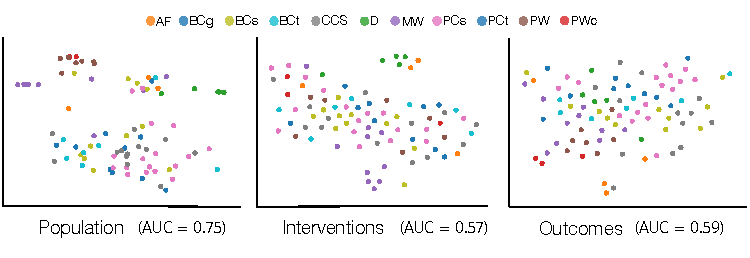
\includegraphics[width=\linewidth]{figures/decisionaidsauc.pdf}
\vspace{-2em}
\caption{TSNE-reduced scatter of disentangled PICO embeddings of abstracts involving ``decision aid" interventions. Abstracts are colored by known population group (see legend). Population embeddings for studies in the same group co-localize, more so than in the intervention and outcome space.}
\label{figure:DATSNE}
\vspace{-.75em}
\end{figure*}

% %sarthak : Changing values to 19K vocab
% \begin{table}
% \small
% \begin{tabularx}{\columnwidth}{X X X X}
% P & I & O & Combined \\ \hline
% 0.75 & 0.57 & 0.59 & 0.70 \\
% \end{tabularx}
% \vspace{-1em}
% \caption{Average pairwise AUCs for decision aids studies under the learned aspect embeddings, calculated w.r.t.~the known population groupings.}
% \label{table:AUCs-DA}
% \vspace{-1em}
% \end{table}

% bcw: IAIN please verify i'm not saying anything stupid
Next we assembled 50 abstracts describing trials involving \emph{hip replacement arthroplasty} (HipRepl). We selected this topic because HipRepl will either describe the trial population (i.e., patients who have received hip replacements) or it will be the intervention, but not both. Thus, we would expect that abstracts describing trials in which HipRepl describes the population cluster in the corresponding embedding space, but not in the intervention space (and vice-versa). To test this, we first manually annotated the 50 abstracts, associating HipRepl with either P or I. We used these labels to calculate pairwise AUCs, reported in Table \ref{table:pubmed-AUCS}. The results imply that the population embeddings discriminate between studies that enrolled patients with HipRepl and other studies. Likewise, studies in which HipRepl was the intervention are grouped in the interventions embedding space, but not in the populations space. 
%As desired, studies labeled as HipRepl Intervention are distinguished from other studies in the I space, but not in the P space; and those %most using intervention embeddings, with similar results for those labeled population.

%sarthak : Changing values to 19K vocab
\begin{table}
\small
\begin{tabularx}{\columnwidth}{c|X X X}
& HipRepl I & HipRepl P & Mean \\ \hline
Population & 0.62 & \textbf{0.68} & \textbf{0.66} \\ 
Intervention & \textbf{0.91} & 0.46 & 0.57 \\ 
Outcome & 0.89 & 0.42 & 0.54 \\ 
% bcw: I think we should just drop O here?
\end{tabularx}
%\vspace{-.65em}
\caption{AUCs realized over HipRepl studies using different embeddings. Column: Study label (HipRepl as P or I). Row: Aspect embedding used.}
\label{table:pubmed-AUCS}
%\vspace{-.75em}
\end{table}

\begin{table}%[h]
\small
\centering
\begin{tabularx}{\columnwidth}{X}
%\hline
%\vspace{-1.25em}
{\bf Population} \emph{american}, \emph{area}, \emph{breast}, \emph{colorectal}, \emph{diagnosis}, \emph{inpatients}, \emph{outpatients}, \emph{stage}, \emph{their}, \emph{uk} \\ \hline
{\bf Intervention} \emph{adjunct}, \emph{alone}, \emph{an}, \emph{discussion}, \emph{intervention}, \emph{methods}, \emph{reduced}, \emph{started}, \emph{took}, \emph{written} \\ \hline
{\bf Outcome} \emph{adults}, \emph{area}, \emph{either}, \emph{eligible}, \emph{importance}, \emph{improve}, \emph{mortality}, \emph{pre}, \emph{reduces}, \emph{survival} \\ %\hline
\end{tabularx}
%\vspace{-1em}
\caption{Top ten most activated words, as determined by the gating mechanism.}
\label{table:picomost}
\vspace{-1em}
\end{table}

\vspace{.15em}
\noindent \textbf{Aspect words}. In Table \ref{table:picomost}, we report the most activated unigrams for each aspect embedding on the decision aids corpus. To derive these we use the outputs of the gating mechanism (Eq. \ref{eq:gate}), which is applied to all words in the input text. For each word, we average the activations across all abstracts and find the top ten words for each aspect. The words align nicely with the PICO aspects, providing further evidence that our model learns to focus on aspect-specific information. % In table \ref{table:highlightpico}, we present an example abstract where each word is highlighted corresponding activations for each aspect. Again, we observe that the activations correspond to our intuition behind which parts of the abstract belong to each aspect.



%%% bcw 12/7 -- have commented out for now anticipating space constraints, but maybe good for supplementary material, or can put back in if space does end up permitting!
\begin{comment}
\begin{figure*}
\minipage{0.32\textwidth}
  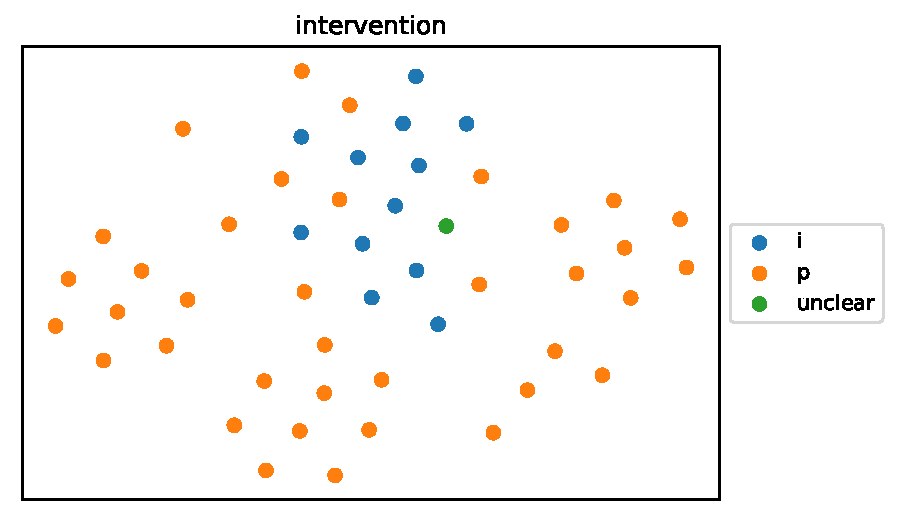
\includegraphics[width=\linewidth]{figures/tsne_pubmed_intervention.pdf}
\endminipage\hfill
\minipage{0.32\textwidth}
  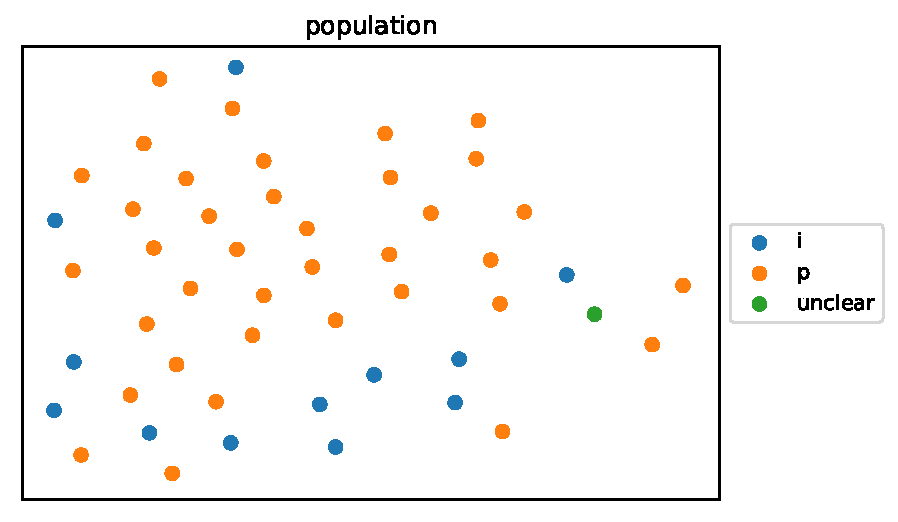
\includegraphics[width=\linewidth]{figures/tsne_pubmed_population.pdf}
\endminipage\hfill
\minipage{0.32\textwidth}%
  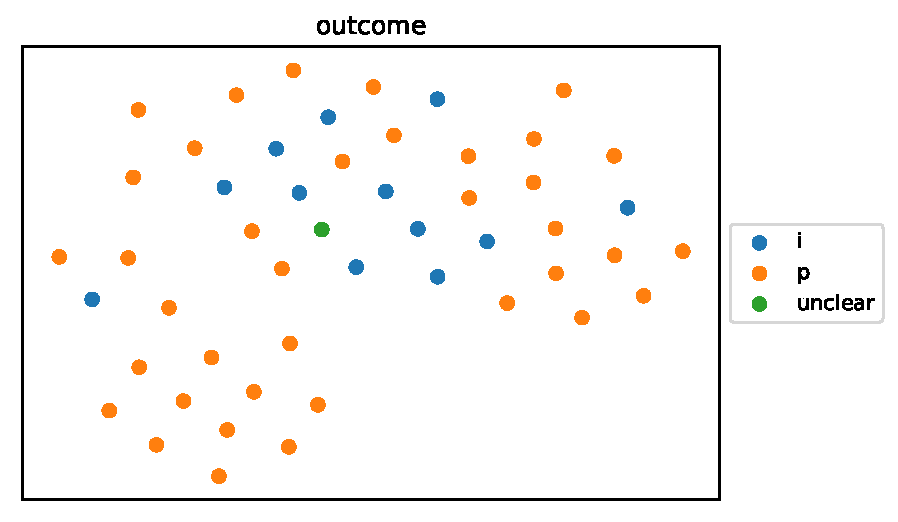
\includegraphics[width=\linewidth]{figures/tsne_pubmed_outcome.pdf}
\endminipage
\end{figure*}

\end{comment}

%\vspace{-.35em}
\subsection{Multi-Aspect Reviews}
%\vspace{-.5em}

We now turn from the specialized domain of biomedical abstracts to more general applications. In particular, we consider learning disentangled representations of beer, hotel and restaurant reviews. Learned embeddings should capture different aspects, e.g., taste or look in the case of beer.

%\vspace{-.2em}
\subsubsection{Beer Reviews (BeerAdvocate)}
%\vspace{-.25em}
\begin{table}%[h]
\setlength{\tabcolsep}{2pt}
\footnotesize
    \centering
    \begin{tabularx}{\columnwidth}{ l X X X X }
     Baseline & Look & Aroma & Palate & Taste  \\
    \hline
    TF-IDF & 0.63 & 0.62 & 0.62 & 0.61  \\
    LDA & 0.73 & 0.73 & 0.73 & 0.73 \\
    Doc2Vec & 0.61 & 0.61 & 0.61 & 0.61  \\
    NVDM & 0.68 & 0.69 & 0.69 & 0.70 \\
    ABAE & 0.50 & 0.50 & 0.50 & 0.50 \\
    \hline
    BoW + Triplet & 0.85 & 0.90 & 0.90 & 0.92 \\
    NVDM + Triplet & 0.90 & 0.91 & 0.92 & 0.95 \\
    DSSM + Triplet &  0.87 & 0.90 & 0.90 & 0.92 \\
    CNN + Triplet & \textbf{0.92} & \textbf{0.93} & \textbf{0.94} & \textbf{0.96} \\
    %\hline
    \end{tabularx}
    %\vspace{-.5em}
    \caption{AUC results for different representations on the BeerAdvocate data. Models beneath the second line are supervised.}
    %\vspace{-.75em}
    \label{table:beerauc}
\end{table}

\begin{table}%[h]
\vspace{-.25em}
\footnotesize
    \centering
    \begin{tabularx}{\columnwidth}{ l X X X X }
     & Look & Aroma & Palate & Taste \\ \hline
    Look & 0.92 & 0.89 & 0.88 & 0.87 \\ 
    Aroma & 0.90 & 0.93 & 0.91 & 0.92 \\ 
    Palate & 0.89 & 0.92 & 0.94 & 0.95 \\ 
    Taste & 0.90 & 0.94 & 0.95 & 0.96 \\ 
    %\hline
    \end{tabularx}
    %\vspace{-.5em}
    \caption{Cross AUC results for different representations on the BeerAdvocate data. Row: Embedding used. Column: Aspect evaluated against. }
    %\vspace{-.75em}
    \label{table:beercrossauc}
\end{table}

\begin{table}%[h]
\setlength{\tabcolsep}{2pt}
\footnotesize
\centering
\begin{tabularx}{\columnwidth}{l|X X|X X|X X|X X}
 & \multicolumn{2}{c|}{Look}  & \multicolumn{2}{c|}{Aroma}  & \multicolumn{2}{c|}{Palate} & \multicolumn{2}{c}{Taste} \\ \hline
Look & - & - & 0.42 &	0.60 & 0.40	& 0.63	& 0.38	& 0.65 \\ %\hline
Aroma & 0.33 & 0.69 & - & - & 0.41 & 0.59 & 0.41 & 0.60 \\ %\hline
Palate & 0.32 & 0.70 & 0.46 & 0.54 & - & - & 0.49 & 0.52 \\ %\hline
Taste & 0.23 & 0.80 & 0.35 & 0.66 & 0.33 & 0.67 & - & - \\
\end{tabularx}
\caption{`Decorrelated' cross-AUC results on the BeerAdvocate data, which attempt to mitigate confounding due to overall sentiment being correlated. Each cell reports metrics over subsets of reviews in which the sentiment differs between the row and column aspects. The numbers in each cell are the AUCs w.r.t. sentiment regarding the column aspect achieved using the row and column aspect representations, respectively.}
\label{table:decorrelated}
\end{table}

We conducted experiments on the BeerAdvocate dataset \cite{mcauley2012learning}, which contains 1.5M reviews of beers that address four aspects: \emph{appearance}, \emph{aroma}, \emph{palate}, and \emph{taste}. Free-text reviews are associated with aspect-specific numerical ratings for each of these, ranging from 1 to 5. We consider ratings $<3$ as negative, and $>3$ as positive, and use these to generate triplets of reviews. For each aspect $a$, we construct triplets $(s, d, o)_a$ by first randomly sampling a review $d$. We then select $s$ to be a review with the same sentiment with respect to $a$ as $d$, and $o$ to be a review with the opposite sentiment regarding $a$. We selected 90K reviews for experiments, such that we had an equal number of positive and negative reviews for each aspect. We only keep words appearing in at least 5 documents, converting all others to $\texttt{unk}$. We truncated reviews to 95 percentile length. We split our data into 80/10/10 ratio for training, validation and testing, respectively. % bcw: again 2000 is kind of low, might raise some eyebrows

\vspace{.25em}
\noindent \textbf{Baselines}. We used the same baselines as for the PICO domain, save for \emph{RR-TF}, which was domain-specific. Here we also evaluate the result of replacing the CNN-based encoder with NVDM, BoW and DSSM based encoders, respectively, each trained using triplet loss.%\footnote{It was unclear how to exploit this supe}

\vspace{.25em}
\noindent  \textbf{Hyperparameters and Settings}. For the CNN-based encoder, we used settings and hyperparameters as described for the PICO domain. For the BoW encoder, we used 800d output embeddings and a PReLU activation function with $\ell_2$ regularization set to $1e$-$5$. For the NVDM based encoder, we used 200d embeddings. % bcw: reviewers may ask how we came to these specific values?

\vspace{.25em}
\noindent \textbf{Metrics}. We again performed an IR-type evaluation to assess the utility of representations. For each aspect $k$, we constructed an affinity matrix $A^k$ such that $A^k_{ij} = {\textit sim}_k(r_i, r_j)$ for beer reviews $r_i$ and $r_j$. We consider two reviews similar under a given aspect $k$ if they have the same (dichotomized) sentiment value for said aspect. We compute AUCs for each review and aspect using the affinity matrix $A_k$. The AUC values are averaged over reviews in the test set to obtain a final AUC metric for each aspect. We also report cross AUC measures in which we use embeddings for aspect $k$ to distinguish reviews under aspect $k'$. % the affinity matrix $A_k$ for aspect $k$ is used to compare against the ground truth for aspect $k'$. That is, 

\vspace{.25em}
\noindent \textbf{Results} We report the AUC measures for each aspect on our test set using different representations in Table \ref{table:beerauc}. Our model consistently outperforms baseline strategies over all aspects. Unsurprisingly, the model outperforms unsupervised approaches.\footnote{We are not sure why ABAE \cite{he-2017} performs so poorly on the review corpora. It may simply fail to prominently encode sentiment, which is important for these tasks. We note that this model performs reasonably well on the PICO data above, and qualitatively seems to recover reasonable aspects (though not specifically sentiment).} We realize consistent though modest improvement over triplet-supervised approaches that use alternative encoders. %though clearly  triplet-loss is more important than the specific encoder architecture used. 

In Table \ref{table:beercrossauc} we present cross AUC evaluations. Rows correspond to the embedding used and columns to the aspect evaluated against. As expected, aspect-embeddings perform better w.r.t.~the aspects for which they code, suggesting some disentanglement. However, the reduction in performance when using one aspect representation to discriminate w.r.t.~others is not as pronounced as above. This is because aspect ratings are highly correlated: if taste is positive, aroma is very likely to be as well. Effectively, here sentiment entangles all of these aspects.\footnote{Another view is that we are in fact inducing representations of $<$aspect, sentiment$>$ pairs, and only the aspect varies across these; thus representations remain discriminative (w.r.t.~sentiment) across aspects.} 

In Table \ref{table:decorrelated}, we evaluate cross AUC performance for beer by first `decorrelating' the aspects. Specifically, for each cell $(k, k')$ in the table, we first retrieve the subset of reviews in which the sentiment w.r.t. $k$ differs from the sentiment w.r.t. $k'$. Then we evaluate the AUC similarity of these reviews on the basis of sentiment concerning $k'$ using both $k$ and $k'$ embeddings, yielding a pair of AUCs (listed respectively). We observe that the using $k'$ embeddings to evaluate aspect $k'$ similarity yields better results than using $k$ embeddings.

We present the most activated words for each aspect (as per the gating mechanism) in Table \ref{table:Beermost}. And we present an illustrative review color-coded with aspect-wise gate activations in Table \ref{table:beer-example}. For completeness, we reproduce the top words for aspects discovered using \newcite{he-2017} in the Appendix; these do not obviously align with the target aspects, which is unsurprising given that this is an unsupervised method.

\begin{table}%[htb]
\vspace{-.5em}
\footnotesize
\centering
\begin{tabularx}{\columnwidth}{X} 
{\bf Look} \emph{attractive}, \emph{beautiful}, \emph{fingers}, \emph{pumpkin}, \emph{quarter}, \emph{received}, \emph{retention}, \emph{sheets}, \emph{sipper}, \emph{well-balanced} \\\hline 
{\bf Aroma} \emph{beer}, \emph{cardboard}, \emph{cheap}, \emph{down}, \emph{follows}, \emph{medium-light}, \emph{rice}, \emph{settled}, \emph{skunked}, \emph{skunky} \\\hline 
{\bf Palate} \emph{bother}, \emph{crafted}, \emph{luscious}, \emph{mellow}, \emph{mint}, \emph{range}, \emph{recommended}, \emph{roasted}, \emph{tasting}, \emph{weight} \\\hline 
{\bf Taste} \emph{amazingly}, \emph{down}, \emph{highly}, \emph{product}, \emph{recommended}, \emph{tasted}, \emph{thoroughly}, \emph{to}, \emph{truly}, \emph{wow} \\
\end{tabularx}
%\vspace{-1em}
\caption{Most activated words for aspects on the beer corpus, as per the gating mechanism.}
\label{table:Beermost}
\vspace{-1em}
\end{table}

\begin{table*}%[h]
\footnotesize
\centering
\begin{tabularx}{\textwidth}{X|X|X|X}
\textbf{Look} : {\setlength{\fboxsep}{0pt}\colorbox{red!99!white}{\strut deep}} {\setlength{\fboxsep}{0pt}\colorbox{red!99!white}{\strut amber}} {\setlength{\fboxsep}{0pt}\colorbox{red!80!white}{\strut hue}} {\setlength{\fboxsep}{0pt}\colorbox{red!58!white}{\strut ,}} {\setlength{\fboxsep}{0pt}\colorbox{red!31!white}{\strut this}} {\setlength{\fboxsep}{0pt}\colorbox{red!34!white}{\strut brew}} {\setlength{\fboxsep}{0pt}\colorbox{red!48!white}{\strut is}} {\setlength{\fboxsep}{0pt}\colorbox{red!75!white}{\strut topped}} {\setlength{\fboxsep}{0pt}\colorbox{red!92!white}{\strut with}} {\setlength{\fboxsep}{0pt}\colorbox{red!99!white}{\strut a}} {\setlength{\fboxsep}{0pt}\colorbox{red!99!white}{\strut finger}} {\setlength{\fboxsep}{0pt}\colorbox{red!99!white}{\strut of}} {\setlength{\fboxsep}{0pt}\colorbox{red!87!white}{\strut off}} {\setlength{\fboxsep}{0pt}\colorbox{red!53!white}{\strut white}} {\setlength{\fboxsep}{0pt}\colorbox{red!20!white}{\strut head}} {\setlength{\fboxsep}{0pt}\colorbox{red!0!white}{\strut .}} {\setlength{\fboxsep}{0pt}\colorbox{red!0!white}{\strut smell}} {\setlength{\fboxsep}{0pt}\colorbox{red!0!white}{\strut of}} {\setlength{\fboxsep}{0pt}\colorbox{red!0!white}{\strut dog}} {\setlength{\fboxsep}{0pt}\colorbox{red!0!white}{\strut unk}} {\setlength{\fboxsep}{0pt}\colorbox{red!0!white}{\strut ,}} {\setlength{\fboxsep}{0pt}\colorbox{red!0!white}{\strut green}} {\setlength{\fboxsep}{0pt}\colorbox{red!0!white}{\strut unk}} {\setlength{\fboxsep}{0pt}\colorbox{red!0!white}{\strut ,}} {\setlength{\fboxsep}{0pt}\colorbox{red!0!white}{\strut and}} {\setlength{\fboxsep}{0pt}\colorbox{red!0!white}{\strut slightly}} {\setlength{\fboxsep}{0pt}\colorbox{red!0!white}{\strut fruity}} {\setlength{\fboxsep}{0pt}\colorbox{red!0!white}{\strut .}} {\setlength{\fboxsep}{0pt}\colorbox{red!27!white}{\strut taste}} {\setlength{\fboxsep}{0pt}\colorbox{red!27!white}{\strut of}} {\setlength{\fboxsep}{0pt}\colorbox{red!27!white}{\strut belgian}} {\setlength{\fboxsep}{0pt}\colorbox{red!0!white}{\strut yeast}} {\setlength{\fboxsep}{0pt}\colorbox{red!0!white}{\strut ,}} {\setlength{\fboxsep}{0pt}\colorbox{red!0!white}{\strut coriander}} {\setlength{\fboxsep}{0pt}\colorbox{red!0!white}{\strut ,}} {\setlength{\fboxsep}{0pt}\colorbox{red!2!white}{\strut hard}} {\setlength{\fboxsep}{0pt}\colorbox{red!5!white}{\strut water}} {\setlength{\fboxsep}{0pt}\colorbox{red!5!white}{\strut and}} {\setlength{\fboxsep}{0pt}\colorbox{red!2!white}{\strut bready}} {\setlength{\fboxsep}{0pt}\colorbox{red!0!white}{\strut malt}} {\setlength{\fboxsep}{0pt}\colorbox{red!0!white}{\strut .}} {\setlength{\fboxsep}{0pt}\colorbox{red!0!white}{\strut light}} {\setlength{\fboxsep}{0pt}\colorbox{red!0!white}{\strut body}} {\setlength{\fboxsep}{0pt}\colorbox{red!0!white}{\strut ,}} {\setlength{\fboxsep}{0pt}\colorbox{red!0!white}{\strut with}} {\setlength{\fboxsep}{0pt}\colorbox{red!31!white}{\strut little}} {\setlength{\fboxsep}{0pt}\colorbox{red!31!white}{\strut carbonation}} {\setlength{\fboxsep}{0pt}\colorbox{red!31!white}{\strut .}} & \textbf{Aroma} : {\setlength{\fboxsep}{0pt}\colorbox{green!1!white}{\strut deep}} {\setlength{\fboxsep}{0pt}\colorbox{green!1!white}{\strut amber}} {\setlength{\fboxsep}{0pt}\colorbox{green!0!white}{\strut hue}} {\setlength{\fboxsep}{0pt}\colorbox{green!0!white}{\strut ,}} {\setlength{\fboxsep}{0pt}\colorbox{green!15!white}{\strut this}} {\setlength{\fboxsep}{0pt}\colorbox{green!16!white}{\strut brew}} {\setlength{\fboxsep}{0pt}\colorbox{green!16!white}{\strut is}} {\setlength{\fboxsep}{0pt}\colorbox{green!0!white}{\strut topped}} {\setlength{\fboxsep}{0pt}\colorbox{green!0!white}{\strut with}} {\setlength{\fboxsep}{0pt}\colorbox{green!3!white}{\strut a}} {\setlength{\fboxsep}{0pt}\colorbox{green!3!white}{\strut finger}} {\setlength{\fboxsep}{0pt}\colorbox{green!3!white}{\strut of}} {\setlength{\fboxsep}{0pt}\colorbox{green!0!white}{\strut off}} {\setlength{\fboxsep}{0pt}\colorbox{green!47!white}{\strut white}} {\setlength{\fboxsep}{0pt}\colorbox{green!47!white}{\strut head}} {\setlength{\fboxsep}{0pt}\colorbox{green!100!white}{\strut .}} {\setlength{\fboxsep}{0pt}\colorbox{green!52!white}{\strut smell}} {\setlength{\fboxsep}{0pt}\colorbox{green!97!white}{\strut of}} {\setlength{\fboxsep}{0pt}\colorbox{green!97!white}{\strut dog}} {\setlength{\fboxsep}{0pt}\colorbox{green!97!white}{\strut unk}} {\setlength{\fboxsep}{0pt}\colorbox{green!51!white}{\strut ,}} {\setlength{\fboxsep}{0pt}\colorbox{green!50!white}{\strut green}} {\setlength{\fboxsep}{0pt}\colorbox{green!53!white}{\strut unk}} {\setlength{\fboxsep}{0pt}\colorbox{green!53!white}{\strut ,}} {\setlength{\fboxsep}{0pt}\colorbox{green!3!white}{\strut and}} {\setlength{\fboxsep}{0pt}\colorbox{green!27!white}{\strut slightly}} {\setlength{\fboxsep}{0pt}\colorbox{green!27!white}{\strut fruity}} {\setlength{\fboxsep}{0pt}\colorbox{green!71!white}{\strut .}} {\setlength{\fboxsep}{0pt}\colorbox{green!58!white}{\strut taste}} {\setlength{\fboxsep}{0pt}\colorbox{green!58!white}{\strut of}} {\setlength{\fboxsep}{0pt}\colorbox{green!13!white}{\strut belgian}} {\setlength{\fboxsep}{0pt}\colorbox{green!0!white}{\strut yeast}} {\setlength{\fboxsep}{0pt}\colorbox{green!0!white}{\strut ,}} {\setlength{\fboxsep}{0pt}\colorbox{green!0!white}{\strut coriander}} {\setlength{\fboxsep}{0pt}\colorbox{green!0!white}{\strut ,}} {\setlength{\fboxsep}{0pt}\colorbox{green!18!white}{\strut hard}} {\setlength{\fboxsep}{0pt}\colorbox{green!18!white}{\strut water}} {\setlength{\fboxsep}{0pt}\colorbox{green!18!white}{\strut and}} {\setlength{\fboxsep}{0pt}\colorbox{green!0!white}{\strut bready}} {\setlength{\fboxsep}{0pt}\colorbox{green!0!white}{\strut malt}} {\setlength{\fboxsep}{0pt}\colorbox{green!0!white}{\strut .}} {\setlength{\fboxsep}{0pt}\colorbox{green!0!white}{\strut light}} {\setlength{\fboxsep}{0pt}\colorbox{green!0!white}{\strut body}} {\setlength{\fboxsep}{0pt}\colorbox{green!0!white}{\strut ,}} {\setlength{\fboxsep}{0pt}\colorbox{green!0!white}{\strut with}} {\setlength{\fboxsep}{0pt}\colorbox{green!52!white}{\strut little}} {\setlength{\fboxsep}{0pt}\colorbox{green!52!white}{\strut carbonation}} {\setlength{\fboxsep}{0pt}\colorbox{green!52!white}{\strut .}} & \textbf{Palate} : {\setlength{\fboxsep}{0pt}\colorbox{cyan!20!white}{\strut deep}} {\setlength{\fboxsep}{0pt}\colorbox{cyan!10!white}{\strut amber}} {\setlength{\fboxsep}{0pt}\colorbox{cyan!33!white}{\strut hue}} {\setlength{\fboxsep}{0pt}\colorbox{cyan!0!white}{\strut ,}} {\setlength{\fboxsep}{0pt}\colorbox{cyan!4!white}{\strut this}} {\setlength{\fboxsep}{0pt}\colorbox{cyan!36!white}{\strut brew}} {\setlength{\fboxsep}{0pt}\colorbox{cyan!39!white}{\strut is}} {\setlength{\fboxsep}{0pt}\colorbox{cyan!34!white}{\strut topped}} {\setlength{\fboxsep}{0pt}\colorbox{cyan!3!white}{\strut with}} {\setlength{\fboxsep}{0pt}\colorbox{cyan!0!white}{\strut a}} {\setlength{\fboxsep}{0pt}\colorbox{cyan!0!white}{\strut finger}} {\setlength{\fboxsep}{0pt}\colorbox{cyan!0!white}{\strut of}} {\setlength{\fboxsep}{0pt}\colorbox{cyan!0!white}{\strut off}} {\setlength{\fboxsep}{0pt}\colorbox{cyan!0!white}{\strut white}} {\setlength{\fboxsep}{0pt}\colorbox{cyan!0!white}{\strut head}} {\setlength{\fboxsep}{0pt}\colorbox{cyan!0!white}{\strut .}} {\setlength{\fboxsep}{0pt}\colorbox{cyan!0!white}{\strut smell}} {\setlength{\fboxsep}{0pt}\colorbox{cyan!0!white}{\strut of}} {\setlength{\fboxsep}{0pt}\colorbox{cyan!0!white}{\strut dog}} {\setlength{\fboxsep}{0pt}\colorbox{cyan!0!white}{\strut unk}} {\setlength{\fboxsep}{0pt}\colorbox{cyan!0!white}{\strut ,}} {\setlength{\fboxsep}{0pt}\colorbox{cyan!0!white}{\strut green}} {\setlength{\fboxsep}{0pt}\colorbox{cyan!0!white}{\strut unk}} {\setlength{\fboxsep}{0pt}\colorbox{cyan!0!white}{\strut ,}} {\setlength{\fboxsep}{0pt}\colorbox{cyan!0!white}{\strut and}} {\setlength{\fboxsep}{0pt}\colorbox{cyan!0!white}{\strut slightly}} {\setlength{\fboxsep}{0pt}\colorbox{cyan!3!white}{\strut fruity}} {\setlength{\fboxsep}{0pt}\colorbox{cyan!3!white}{\strut .}} {\setlength{\fboxsep}{0pt}\colorbox{cyan!5!white}{\strut taste}} {\setlength{\fboxsep}{0pt}\colorbox{cyan!1!white}{\strut of}} {\setlength{\fboxsep}{0pt}\colorbox{cyan!1!white}{\strut belgian}} {\setlength{\fboxsep}{0pt}\colorbox{cyan!0!white}{\strut yeast}} {\setlength{\fboxsep}{0pt}\colorbox{cyan!0!white}{\strut ,}} {\setlength{\fboxsep}{0pt}\colorbox{cyan!2!white}{\strut coriander}} {\setlength{\fboxsep}{0pt}\colorbox{cyan!35!white}{\strut ,}} {\setlength{\fboxsep}{0pt}\colorbox{cyan!69!white}{\strut hard}} {\setlength{\fboxsep}{0pt}\colorbox{cyan!98!white}{\strut water}} {\setlength{\fboxsep}{0pt}\colorbox{cyan!64!white}{\strut and}} {\setlength{\fboxsep}{0pt}\colorbox{cyan!31!white}{\strut bready}} {\setlength{\fboxsep}{0pt}\colorbox{cyan!33!white}{\strut malt}} {\setlength{\fboxsep}{0pt}\colorbox{cyan!66!white}{\strut .}} {\setlength{\fboxsep}{0pt}\colorbox{cyan!100!white}{\strut light}} {\setlength{\fboxsep}{0pt}\colorbox{cyan!99!white}{\strut body}} {\setlength{\fboxsep}{0pt}\colorbox{cyan!99!white}{\strut ,}} {\setlength{\fboxsep}{0pt}\colorbox{cyan!99!white}{\strut with}} {\setlength{\fboxsep}{0pt}\colorbox{cyan!99!white}{\strut little}} {\setlength{\fboxsep}{0pt}\colorbox{cyan!98!white}{\strut carbonation}} {\setlength{\fboxsep}{0pt}\colorbox{cyan!65!white}{\strut .}} & \textbf{Taste} :{\setlength{\fboxsep}{0pt}\colorbox{yellow!40!white}{\strut deep}} {\setlength{\fboxsep}{0pt}\colorbox{yellow!42!white}{\strut amber}} {\setlength{\fboxsep}{0pt}\colorbox{yellow!12!white}{\strut hue}} {\setlength{\fboxsep}{0pt}\colorbox{yellow!6!white}{\strut ,}} {\setlength{\fboxsep}{0pt}\colorbox{yellow!49!white}{\strut this}} {\setlength{\fboxsep}{0pt}\colorbox{yellow!94!white}{\strut brew}} {\setlength{\fboxsep}{0pt}\colorbox{yellow!100!white}{\strut is}} {\setlength{\fboxsep}{0pt}\colorbox{yellow!55!white}{\strut topped}} {\setlength{\fboxsep}{0pt}\colorbox{yellow!10!white}{\strut with}} {\setlength{\fboxsep}{0pt}\colorbox{yellow!4!white}{\strut a}} {\setlength{\fboxsep}{0pt}\colorbox{yellow!4!white}{\strut finger}} {\setlength{\fboxsep}{0pt}\colorbox{yellow!4!white}{\strut of}} {\setlength{\fboxsep}{0pt}\colorbox{yellow!0!white}{\strut off}} {\setlength{\fboxsep}{0pt}\colorbox{yellow!0!white}{\strut white}} {\setlength{\fboxsep}{0pt}\colorbox{yellow!0!white}{\strut head}} {\setlength{\fboxsep}{0pt}\colorbox{yellow!11!white}{\strut .}} {\setlength{\fboxsep}{0pt}\colorbox{yellow!11!white}{\strut smell}} {\setlength{\fboxsep}{0pt}\colorbox{yellow!53!white}{\strut of}} {\setlength{\fboxsep}{0pt}\colorbox{yellow!43!white}{\strut dog}} {\setlength{\fboxsep}{0pt}\colorbox{yellow!43!white}{\strut unk}} {\setlength{\fboxsep}{0pt}\colorbox{yellow!34!white}{\strut ,}} {\setlength{\fboxsep}{0pt}\colorbox{yellow!35!white}{\strut green}} {\setlength{\fboxsep}{0pt}\colorbox{yellow!37!white}{\strut unk}} {\setlength{\fboxsep}{0pt}\colorbox{yellow!3!white}{\strut ,}} {\setlength{\fboxsep}{0pt}\colorbox{yellow!41!white}{\strut and}} {\setlength{\fboxsep}{0pt}\colorbox{yellow!39!white}{\strut slightly}} {\setlength{\fboxsep}{0pt}\colorbox{yellow!39!white}{\strut fruity}} {\setlength{\fboxsep}{0pt}\colorbox{yellow!0!white}{\strut .}} {\setlength{\fboxsep}{0pt}\colorbox{yellow!0!white}{\strut taste}} {\setlength{\fboxsep}{0pt}\colorbox{yellow!44!white}{\strut of}} {\setlength{\fboxsep}{0pt}\colorbox{yellow!48!white}{\strut belgian}} {\setlength{\fboxsep}{0pt}\colorbox{yellow!48!white}{\strut yeast}} {\setlength{\fboxsep}{0pt}\colorbox{yellow!6!white}{\strut ,}} {\setlength{\fboxsep}{0pt}\colorbox{yellow!35!white}{\strut coriander}} {\setlength{\fboxsep}{0pt}\colorbox{yellow!66!white}{\strut ,}} {\setlength{\fboxsep}{0pt}\colorbox{yellow!94!white}{\strut hard}} {\setlength{\fboxsep}{0pt}\colorbox{yellow!61!white}{\strut water}} {\setlength{\fboxsep}{0pt}\colorbox{yellow!29!white}{\strut and}} {\setlength{\fboxsep}{0pt}\colorbox{yellow!4!white}{\strut bready}} {\setlength{\fboxsep}{0pt}\colorbox{yellow!15!white}{\strut malt}} {\setlength{\fboxsep}{0pt}\colorbox{yellow!35!white}{\strut .}} {\setlength{\fboxsep}{0pt}\colorbox{yellow!70!white}{\strut light}} {\setlength{\fboxsep}{0pt}\colorbox{yellow!58!white}{\strut body}} {\setlength{\fboxsep}{0pt}\colorbox{yellow!38!white}{\strut ,}} {\setlength{\fboxsep}{0pt}\colorbox{yellow!2!white}{\strut with}} {\setlength{\fboxsep}{0pt}\colorbox{yellow!19!white}{\strut little}} {\setlength{\fboxsep}{0pt}\colorbox{yellow!20!white}{\strut carbonation}} {\setlength{\fboxsep}{0pt}\colorbox{yellow!17!white}{\strut .}}
\end{tabularx}
%\vspace{-.75em}
\caption{Gate activations for each aspect in an example beer review. }
\label{table:beer-example}
%\vspace{-.75em}
\end{table*} 

%\vspace{-.3em}
\subsubsection{Hotel \& Restaurant Reviews}
%\vspace{-.25em}

%The TripAdvisor data includes reviews of hotels with ratings (range 1 to 5). The Yelp! corpus includes restaurant reviews on the same scale.
Finally, we attempt to learn embeddings that disentangle domain from sentiment in reviews. For this we use a combination of TripAdvisor and Yelp! ratings data. The former comprises reviews of hotels, the latter of restaurants; both use a scale of 1 to 5. We convert ratings into positive/negative labels as above. Here we consider aspects to be the domain (hotel or restaurant) and the sentiment (positive or negative). We aim to generate embeddings that capture information about only one of these aspects. We use 50K reviews from each dataset for training and 5K for testing. 
% about the domain (restaurant vs hotel) or sentiment (positive vs negative)

\vspace{.2em}
\noindent \textbf{Baselines}. We use the same baselines as for the BeerAdvocate data, and similarly use different encoder models trained under triplet loss.

\begin{table}
\footnotesize
    \centering
    \begin{tabularx}{\columnwidth}{l X X}
     Baseline & Domain & Sentiment  \\
    \hline
    TF-IDF & 0.59 & 0.52   \\
    Doc2Vec & 0.83 & 0.56 \\
    LDA & 0.90 & 0.62 \\
    NVDM & 0.79 & 0.63  \\
    ABAE & 0.50 & 0.50 \\
    \hline
    BoW + Triplet & \textbf{0.99} & 0.91 \\
    NVDM + Triplet & \textbf{0.99} & 0.91 \\
    DSSM + Triplet &  \textbf{0.99} & 0.90 \\
    CNN + Triplet & \textbf{0.99} & \textbf{0.92}  \\
    \end{tabularx}
    %\vspace{-.75em}
    \caption{AUC results for different representations on the Yelp!/TripAdvisor Data. Models beneath the second line are supervised.}
    %\vspace{-.25em}
    \label{table:foodauc}
\end{table}

\vspace{.2em}
\noindent \textbf{Evaluation Metrics}. We perform AUC and cross-AUC evaluation as in the preceding section. For the domain aspect, we consider two reviews similar if they are from the same domain, irrespective of sentiment. Similarly, reviews are considered similar with respect to the sentiment aspect if they share a sentiment value, regardless of domain.

%With respect to the sentiment aspect, reviews are considered similar if they have the same sentiment value (regardless of the domain).%irrespective of its domain.

% We construct for each aspect a similarity matrix $S^k_{ij}$ on complete test set. The similarity matrix $S^k$ for each aspect $k$ is defined as $S^k_{ij} = sim_k(a_i, a_j)$ for all pairs of reviews $a_i$ and $a_j$. For each review $a_i$, we calculate its ROC curve under aspect $k$ and average over the AUC values over all reviews, to get a single AUC score for aspect $k$.

% Similar to BeerAdvocate domain, we also compute cross-AUC values using affinity matrices $A^{kk'}_{ij}$ for given aspect $k$ is constructed using embeddings for aspect $k'$.



\begin{table}%[h]
\footnotesize
    \centering
    \begin{tabularx}{\columnwidth}{l X X}
     Baseline & Domain & Sentiment  \\
    \hline
    Domain & 0.988 & 0.512   \\
    Sentiment & 0.510 & 0.917  \\
    %\hline
    \end{tabularx}
    %\vspace{-.75em}
    \caption{Cross AUC results for different representations for Yelp!/TripAdvisor Dataset.}
    %\vspace{-1.0em}
    \label{table:foodcrossauc}
\end{table}

\vspace{.25em}
\noindent  \textbf{Results}. In Table \ref{table:foodauc} we report the AUCs for each aspect on our test set using different representations. Baselines perform reasonably well on the domain aspect because reviews from different domains are quite dissimilar. Capturing sentiment information irrespective of domain is more difficult, and most unsupervised models fail in this respect. In Table \ref{table:foodcrossauc}, we observe that cross AUC results are much more pronounced than for the BeerAdvocate data, as the domain and sentiment are uncorrelated (i.e., sentiment is independent of domain).

%\vspace{-.5em}
\section{Related Work}
%\vspace{-.5em}
\label{section:related-work}
%Neural models capitalize on dense, distributed representations (i.e., embeddings) that represent individual words \cite{mikolov2013distributed} or other linguistic units such as sentences \cite{le2014distributed}. Intuitively, such embeddings encode a \emph{distributional semantics} \cite{firth1957synopsis}: similar words (or sentences) will be placed nearby one another in the embedding space.

Work in representation learning for NLP has largely focused on improving word embeddings \cite{levy2014dependency,faruqui2014retrofitting,huang2012improving}. But efforts have also been made to embed other textual units, e.g. characters \cite{kim2016character}, and lengthier texts including sentences, paragraphs, and documents \cite{le2014distributed,kiros2015skip}. 

Triplet-based judgments have been used in multiple domains, including vision and NLP, to estimate similarity information implicitly. For example, triplet-based similarity embeddings may be learned using `crowdkernels' with applications to multi-view clustering \cite{amid2015multiview}. Models combining similarity with neural networks mainly revolve around Siamese networks \cite{chopra2005learning} which use pairwise distances to learn embeddings \cite{schroff2015facenet}, a tactic we have followed here. Similarity judgments have also been used to generate document embeddings for IR tasks \cite{shen2014latent,das2016together}.%, although here judgments tend specify where individual pairs are similar or dissimilar.

Recently, \newcite{he-2017} introduced a neural model for aspect extraction that relies on an attention mechanism to identify aspect words. They proposed an autoencoder variant designed to tease apart aspects. In contrast to the method we propose, their approach is unsupervised; discovered aspects may thus not have a clear interpretation. Experiments reported here support this hypothesis, and we provide additional results using their model in the Appendix. 



%(nor is there an obvious way to guide estimation of target aspects of interest). %\newcite{zhang2017aspect}

%They first induce a sentence embedding $z_s$ and then attempt to reconstruct this via a simple autoencoder which is designed to explicitly tease apart aspects. More specifically, the decoder component of the model reconstructs the input sentence via a linear combination of latent aspect embedding representations. To discourage redundancy between the learned aspects, they introduced a regularization penalty that explicitly encourages aspect embedding diversity. They were able to uncover meaningful aspects from text using this method. 

Other recent work has focused on text \emph{generation} from factorized representations \cite{larsson2017disentangled}. And \newcite{zhang2017aspect} proposed a lightly supervised method for \emph{domain adaptation} using aspect-augmented neural networks. They exploited \emph{source} document labels to train a classifier for a \emph{target} aspect. They leveraged sentence-level scores codifying sentence relevance w.r.t.~individual aspects, which were derived from terms \emph{a priori} associated with aspects. This supervision is used to construct a composite loss that captures both classification performance on the source task and a term that enforces \emph{invariance} between source and target representations.

%They use this supervision to induce aspect-specific representations of input texts by minimizing a loss that includes terms capturing classification performance on the source task, and an adversarial loss that attempts to enforce invariance between representations of source and target representations. 

%On the other hand, in many tasks we cannot explicitly label or even define discrete values for a given aspect whereas similarity judgments are easier to obtain.

There is also a large body of work that uses probabilistic generative models to recover latent structure in texts. Many of these models derive from Latent Dirichlet Allocation (LDA) \cite{blei2003latent}, and some variants have explicitly represented topics and aspects jointly for sentiment tasks \cite{brody2010unsupervised,sauper2010incorporating,sauper2011content,mukherjee2012aspect,sauper2013automatic,kim2013hierarchical}. 

A bit more generally, \emph{aspects} have also been interpreted as properties spanning entire texts, e.g., a perspective or theme which may then color the discussion of topics \cite{paul2010two}. This intuition led to the development of the \emph{factorial LDA} family of topic models \cite{paul2012factorial,wallace2014large}; these model individual word probability as a product of multiple latent factors characterizing a text. This is similar to the Sparse Additive Generative (SAGE) model of text proposed by \newcite{SAGE}.%Eisenstein \cite{SAGE}. 

% bcw: not sure we need this stuff, since focus not on auto-encoders here
%Several neural approaches to document modeling have recently been proposed, including the Neural Variational Document Model (NVDM) \cite{miao2016neural}, autoencoding LDA, and extensions thereof \cite{srivastava2017autoencoding}. The above models all learn a representation $z \in R^K$ of a document in which each component $z_k$ is associated with a vector $\beta_k$ of log-frequencies (NVDM) or probabilities (autoencoding LDA) that encodes a topic. This representation is entangled in the sense that we would generally not expect to be able to identify subsets of topics pertaining to specific aspects.

%\vspace{-.25em}
\section{Conclusions}
%\vspace{-.5em}

We have proposed an approach for inducing disentangled representations of text. To learn such representations we have relied on supervision codified in aspect-wise similarity judgments expressed as document triplets. This provides a general supervision framework and objective. We evaluated this approach on three datasets, each with different aspects. Our experimental results demonstrate that this approach indeed induces aspect-specific embeddings that are qualitatively interpretable and achieve superior performance on information retrieval tasks. 

Going forward, disentangled representations may afford additional advantages in NLP, e.g., by facilitating transfer \cite{zhang2017aspect}, or supporting aspect-focused summarization models. 


\section{Acknowledgements}
This work was supported by National Library of Medicine (NLM) of the National Institutes of Health (NIH) award R01LM012086, and by the Army Research Office (ARO) award W911NF1810328. The content is solely the responsibility of the authors.


\bibliography{emnlp2018}
\bibliographystyle{acl_natbib_nourl}

\end{document}
